\documentclass[journal]{./IEEE/IEEEtran}
\usepackage{cite,graphicx}
\usepackage{float}
\usepackage{makeidx}

\newcommand{\SPTITLE}{3D Mobile Simulation Application for Learning Seasonal Beehive Management}
\newcommand{\ADVISEE}{Albert Dominic Crisostomo}
\newcommand{\ADVISER}{Prof. Arian J. Jacildo}

\newcommand{\BSCS}{Bachelor of Science in Computer Science}
\newcommand{\ICS}{Institute of Computer Science}
\newcommand{\UPLB}{University of the Philippines Los Ba\~{n}os}
\newcommand{\REMARK}{\thanks{Presented to the Faculty of the \ICS, \UPLB\
                             in partial fulfillment of the requirements
                             for the Degree of \BSCS}}
        
\markboth{CMSC 190 Special Problem, \ICS}{}
\title{\SPTITLE}
\author{\ADVISEE~and~\ADVISER%
\REMARK
}
% fix this vvvvv
\pubid{\copyright~2019~ICS \UPLB}

%%%%%%%%%%%%%%%%%%%%%%%%%%%%%%%%%%%%%%%%%%%%%%%%%%%%%%%%%%%%%%%%%%%%%%%%%%
\begin{document}

% TITLE
\maketitle

\begin{abstract}
    The UPLB Bee Program offers the Intensive Beekeeping Course in which beekeeping experts teach the fundamentals of honey bee rearing, beehive management, and efficient production of honey. The objectives of this study were to provide another way to teach the fundamentals and explore mobile technologies by developing a mobile simulation application. A working mobile simulation application was developed, and was successful in rendering 3D models of beehive elements. Automatic beekeeping simulation was also developed along with the manual beekeeping. A quiz mode was developed to facilitate quizzes about frame types for users. It has simulated both proper and improper seasonal beehive management, and provided interactive quiz sets for users.
    \newline
    \newline \indent
    \emph{Index Terms---} Beehive Management, Simulation, 3D Models, Mobile Technologies
\end{abstract}

% INTRODUCTION
\section{Introduction}
\indent The UPLB Bee Program "is a multi-disciplinary, integrated, research and extension program established in 1989 to promote, formalize and integrate all bee-related research and extension activities of UPLB" \cite{uplbbeeprogram}. It employs extension programming which includes trainings, technical services, and technology promotion. Currently, its trainings include Intensive Beekeeping Course, Management of Tropical Bees, and Product Development \cite{uplbbeeprogramsite}. The Intensive Beekeeping Course in particular uses a combination of lectures, demonstrations, laboratory and field work, and video showing, and maintains the hands-on activities as comprising bulk of the Course \cite{beekeepingtraining}.
\newline
\indent One of the modules of the trainings is the seasonal beehive management which currently uses a series of presentation slides for demonstration. There were attempts in the past to develop a 3D simulation of seasonal beehive management \cite{serrano}\cite{clarino}. All of them were developed only for desktop computers. However, this study will explore current 3D technologies in mobile devices.
\newline
\indent Simulation is a branch of computer science that is defined as a representation of the main features of a system \cite{naziretal}. It was first used as a military simulation in the 1960s. Since then, it has become a wide field of knowledge and is used for different purposes such as education, scientific modeling, video games, introduction to new technology, and so on \cite{naziretal}. The continuous advancements in computer hardware and software enabled the development of more sophisticated and interactive simulation environments. These environments are designed to allow users to experiment with different parameters and then analyze the outcomes after some interactions, giving the users the opportunity to improve their decision-making capabilities \cite{barbosa}. 
\newline
\indent 3D simulation aims to represent the functionalities of a proposed physical system, while creating visual models that appear realistic. Due to its nature, developers have more room to improve interactivity and visual aesthetics of their simulations, subsequently engaging more people to learn and observe \cite{santosaetal}.
\newline
\indent Beehive management, also known as beekeeping, is the management man-made beehives in order to expand the residing bee colonies and eventually harvest honey from them \cite{bradbear}. Bees in their natural habitats have contributed to the proliferation of various species of flowering plants and crops. Bee species that are nurtured for beekeeping purposes are also capable of doing such feat; thus, their honey gathering routine is beneficial to the natural environment, including forests \cite{agera}. Beekeeping produces honey and beeswax, which can be made into various products. Some of those products are candles, cosmetic and skin care products, herbal medicines (propolis), and royal jelly.
\newline
\indent Smartphones are becoming more and more ubiquitous. It began from simple tasks such as sending and receiving SMS texts from one phone to another, to more sophisticated and complex tasks such as providing access to the Internet, interact with various kinds of mobile applications, and so on. One kind of those applications is mobile games.
\newline
\indent Generally, mobile games are consumed by end-users for entertainment. Most of the developers of these games implement the “freemium” model to generate income from their consumers. This business model enacts the development of a free-to-play mobile game with in-app purchases \cite{heier}. However, there are still some games that do not use this model, offering only a free-to-play mobile game. Some of them are “serious games,” which are games that offer not only entertainment but also some other form of incentive, in general.  Specifically, mobile serious games can be those that offer not only entertainment, but also learnings from a field of knowledge \cite{sugimuraetal}.
\newline
\pubidadjcol
\indent Previous studies were conducted to develop a 3D simulation tool of seasonal beehive management for desktop computers \cite{serrano}\cite{clarino}. In 2011, Serrano simulated seasonal beehive management in a span of one (1) Beekeeping Season. Moreover, it allows users to observe the behavior of the beehive and interact with the beehive and its frame housing for bees. Lastly, the 3D simulation tool displays resulting data derived from the users{'} actions and interactions with the frames inside the beehive. On the other hand, Clari\~{n}o developed a desktop 3D simulation tool of the same topic, subsequent to Serrano{'}s study \cite{clarino}. He created features whose functionalities are similar to some of Serrano{'}s, but also added a new feature.
\newline 
\indent Serrano{'}s and Clari\~{n}o{'}s studies were successful in laying the foundation for the development of 3D seasonal beehive management simulation. However, their simulation tools were developed only for desktop computers, which is the studies’ gap given the current trend of computer technologies.

% OBJECTIVES
\section{Objectives}
The main objective of this study is to develop a 3D mobile simulation application that allows 3D simulation and interaction with seasonal beehive management. It teaches the users proper beehive practices and simulates the outcomes of proper and improper practices. Specifically, the study aims to:
\begin{enumerate}
    \item identify the relevant seasonal beehive management elements which are food frames and boxes;
    \item create 3D objects from the identified elements and provide UI to interact with these objects;
    \item deploy the developed 3D mobile simulation application to Android OS; and
    \item improve the accuracy and precision of the simulations and outcomes of the player{'}s interaction with the application.
\end{enumerate}

% METHODOLOGY
\section{Methodology}
\indent Blender was used in creating the 3D models such as the wired frame and the Langstroth boxed hive, based on the specifications provided by the UPLB Bee Program \cite{cervanciaetal}. The game engine Unity3D was used in developing the simulation app. C\# was the programming language used for implementing the simulation logic and other back-end functionalities.
\subsection{Elements}
\pubidadjcol
The elements found in the simulation are the frames, bees, and boxed hive. The frames are where bees form the honeycombs. The boxed hive is where all the frames will be placed in. The bees are the ones gathering food, feeding the brood, and creating sticky frames. The following are five types of frames:
\begin{itemize}
    \item \textit{Food Frame}: it contains food.
    \item \textit{Open Brood Frame}: it consists of egg or larvae.
    \item \textit{Sealed Brood Frame}: it is composed of pupa.
    \item \textit{Sticky Frame}: it contains honeycomb.
    \item \textit{Foundation Frame}: it is constructed with wax foundation for bees to build honeycomb.
\end{itemize}
\subsection{Process Flows}
When a new frame is added, it is a foundation frame. In 14 days (in-app), the bees will transform it into a sticky frame. The sticky frame can transform into an open brood frame. If it becomes an open brood frame, the eggs/larvae will transform into pupa after 9 days turning the frame into a sealed brood frame. After 12 days, the pupa will fully mature into adult bees leaving the frame empty making it a sticky frame. Fig. 1 illustrates the frame cycle.
\begin{figure}[H]
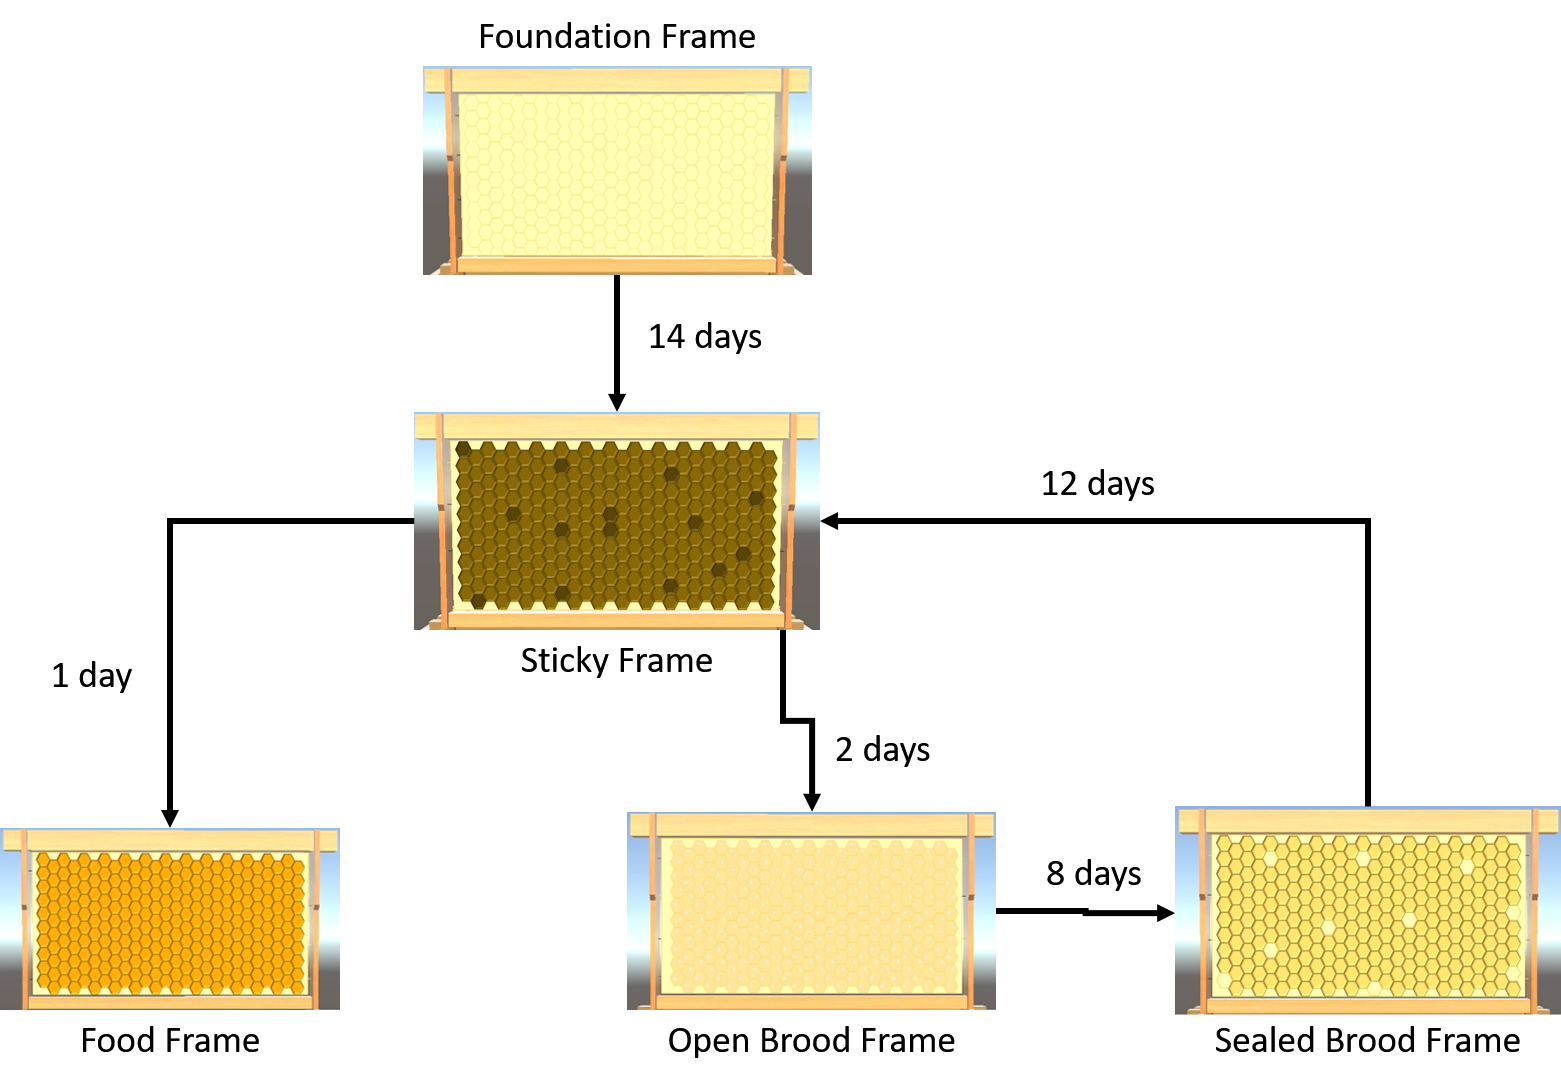
\includegraphics[scale=0.3]{./images/frame-cycle.png}
\centering
\caption{Flowchart of frame cycle}
\end{figure}
\indent

The following are the steps for Proper Seasonal Beehive Management:
\begin{enumerate}
    \item Make a nucleus colony.
    \item Place Foundation Frames to expand colony.
    \item Place Food Frames to feed colony.
    \item Keep Brood frames in the relative center of the hive.
    \item Place new Sticky Frames in the relative center for the queen to lay eggs in.
    \item If there is too little food, place Food Frame.
    \item Repeat Step 2 until the colony has 10 Frames.
\end{enumerate}
\indent Below are some of the Improper Beehive Management practices, such as:
\begin{itemize}
    \item not placing Foundation Frames;
    \item adding Foundation Frames too soon or too late; and
    \item placing Sticky Frames in unsuitable locations.
\end{itemize}

\subsection{User Interface}
\indent
The mobile simulation application contains 4 scenes, i.e. the Main Menu, the Quiz, the Automatic Beekeeping, and the Manual Beekeeping as shown in Fig. 2, Fig. 3, Fig. 4, and Fig. 5. Each scene contains different UI elements, while the functionalities of some elements are shared among the scenes. Below are the UI elements developed in the mobile app:
\begin{itemize}
    \item \textit{Automatic Beekeeping}: It is a button that allows the user to observe automatic simulation of proper beehive management.
    \item \textit{Manual Beekeeping}: It is a button that allows the user to manually interact with the beehive.
    \item \textit{Quiz}: It is a button that facilitates a quiz about frame types for the user.
    \item \textit{Set 1}: It is a button that loads the frames in a proper setup.
    \item \textit{Set 2}: It is a button that loads the frames in an improper setup.
    \item \textit{Set 3}: It is a button that loads the frames in another improper setup.
    \item \textit{Reset}: It restores the current state of the Set back to its original one.
    \item \textit{Score Label}: It displays the current score of the user in a current Set.
    \item \textit{Raise All Frames}: It is a button that lifts all present frame above the boxed hive.
    \item \textit{Lower All Frames}: It lowers all present frame above the boxed hive.
    \item \textit{Move Frame to Back}: It is a button that moves currently selected frame backwards.
    \item \textit{Move Frame to Front}: It moves currently selected frame to the front of the boxed hive.
    \item \textit{Move Frame to Back}: It is a button that moves currently selected frame backwards.
    \item \textit{Raise Frame}: It is a button that lifts the currently selected frame.
    \item \textit{Lower Frame}: It is a button that lowers the currently selected frame.
    \item \textit{Simulate}: It starts the automatic simulation of proper seasonal beehive management.
    \item \textit{Toggle Graph}: It is a button that toggles the visibility of the Graph.
    \item \textit{Graph}: It is a line graph feature that displays the total population of bees per in-app day.
    \item \textit{Monitor}: It is a group of text labels which displays the current Day, Food count, Egg count, Pupa count, Worker count, and Total Population.
    \item \textit{Foundation Frame}: It is a button that renders a Foundation Frame at the nearest available spot of the boxed hive.
    \item \textit{Open Brood Frame}: It renders an Open Brood Frame.
    \item \textit{Sealed Brood Frame}: It renders a Sealed Brood Frame at the nearest available spot of the boxed hive.
    \item \textit{Sticky Frame}: It renders a Sticky Frame at the nearest available spot of the boxed hive.
    \item \textit{Food Frame}: It renders a Food Frame at the nearest available spot of the boxed hive.
    \item \textit{Pause/Play}: It is a button that pauses or resumes the progress of automatic beehive management.
    \item \textit{Simulation Speed Button}: It is a a group of buttons that change the speed of the simulation.
    \item \textit{Next Day}: It is a button that proceeds the manual simulation towards the next in-app day.
    \item \textit{Exit Apis}: It is a button that exits the scene.
    \item \textit{Quit}: It is a button that closes the mobile application.
\end{itemize}

\begin{figure}[H]
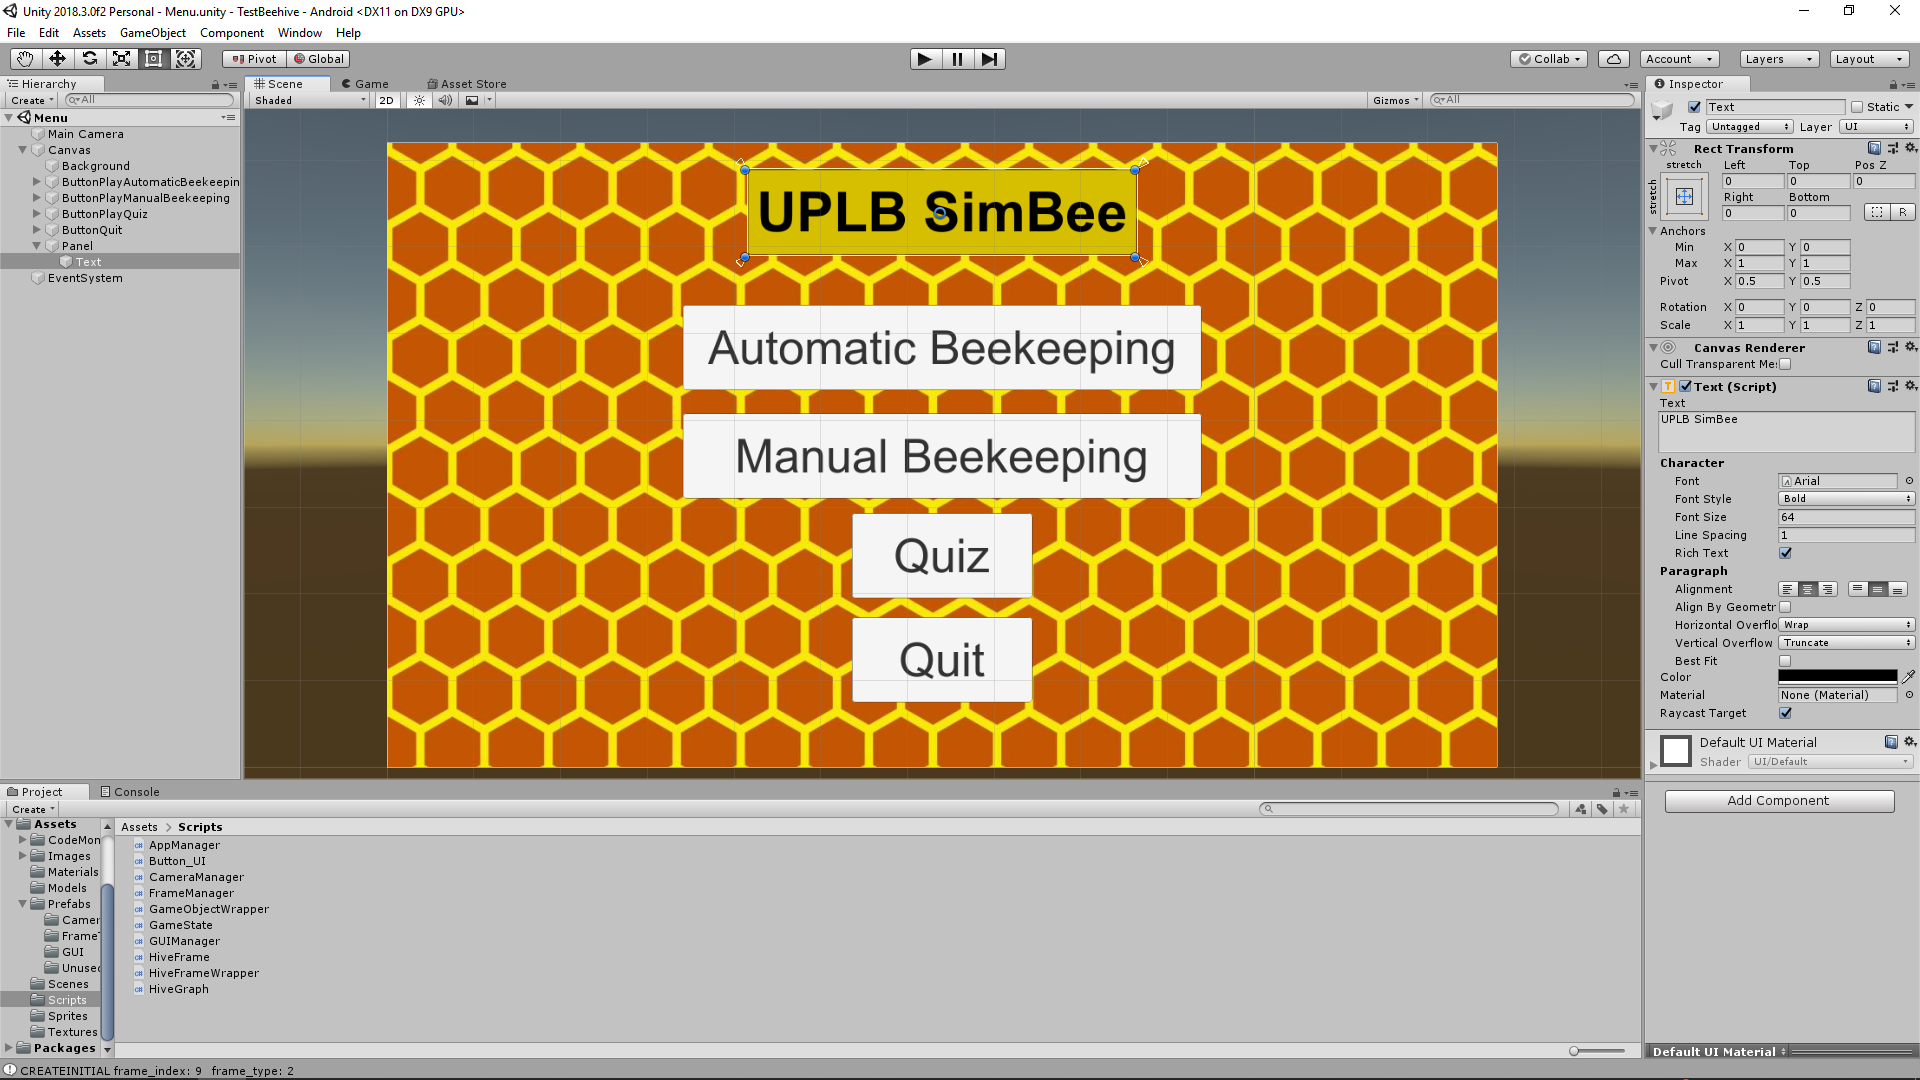
\includegraphics[scale=0.15]{./images/ui-menu.png}
\centering
\caption{The development of Main Menu UI}
\centering
\end{figure}

\begin{figure}[H]
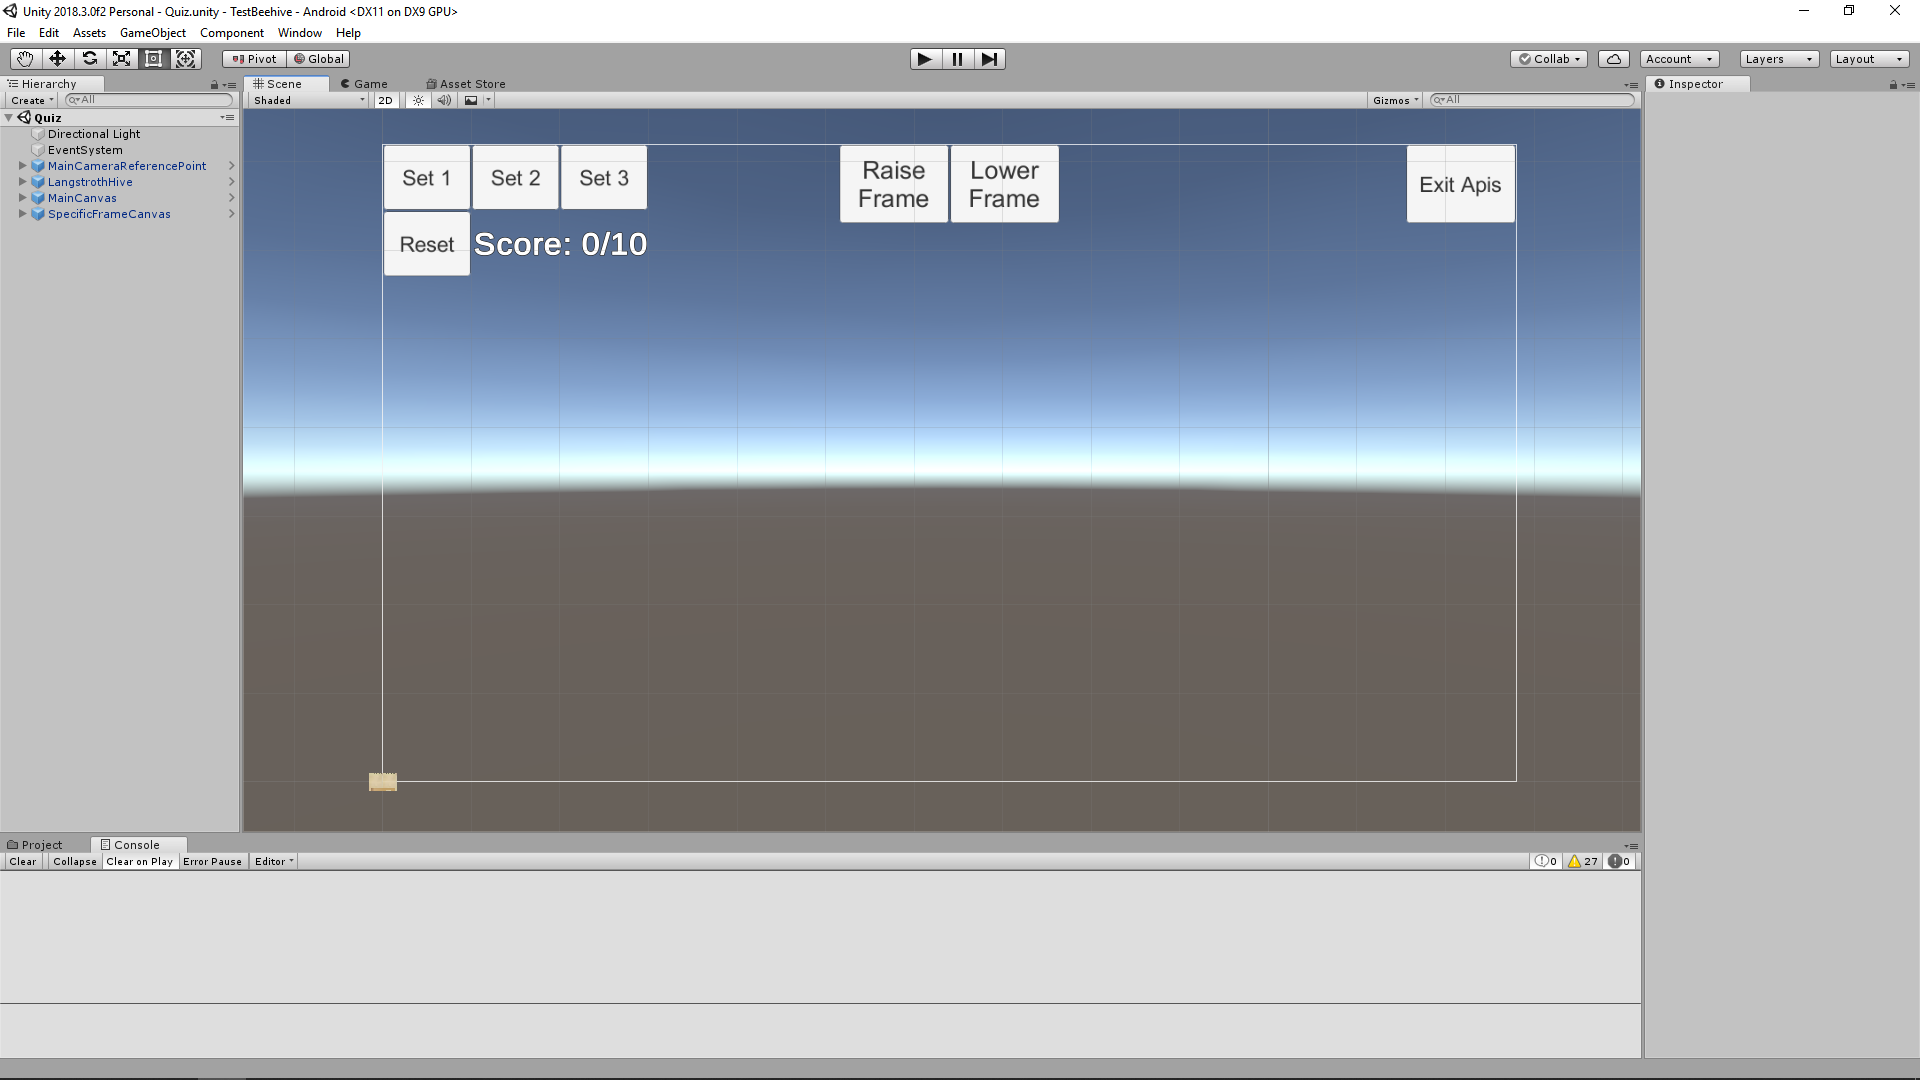
\includegraphics[scale=0.15]{./images/new-quiz-ui.png}
\centering
\caption{The development of Quiz UI}
\centering
\end{figure}

\begin{figure}[H]
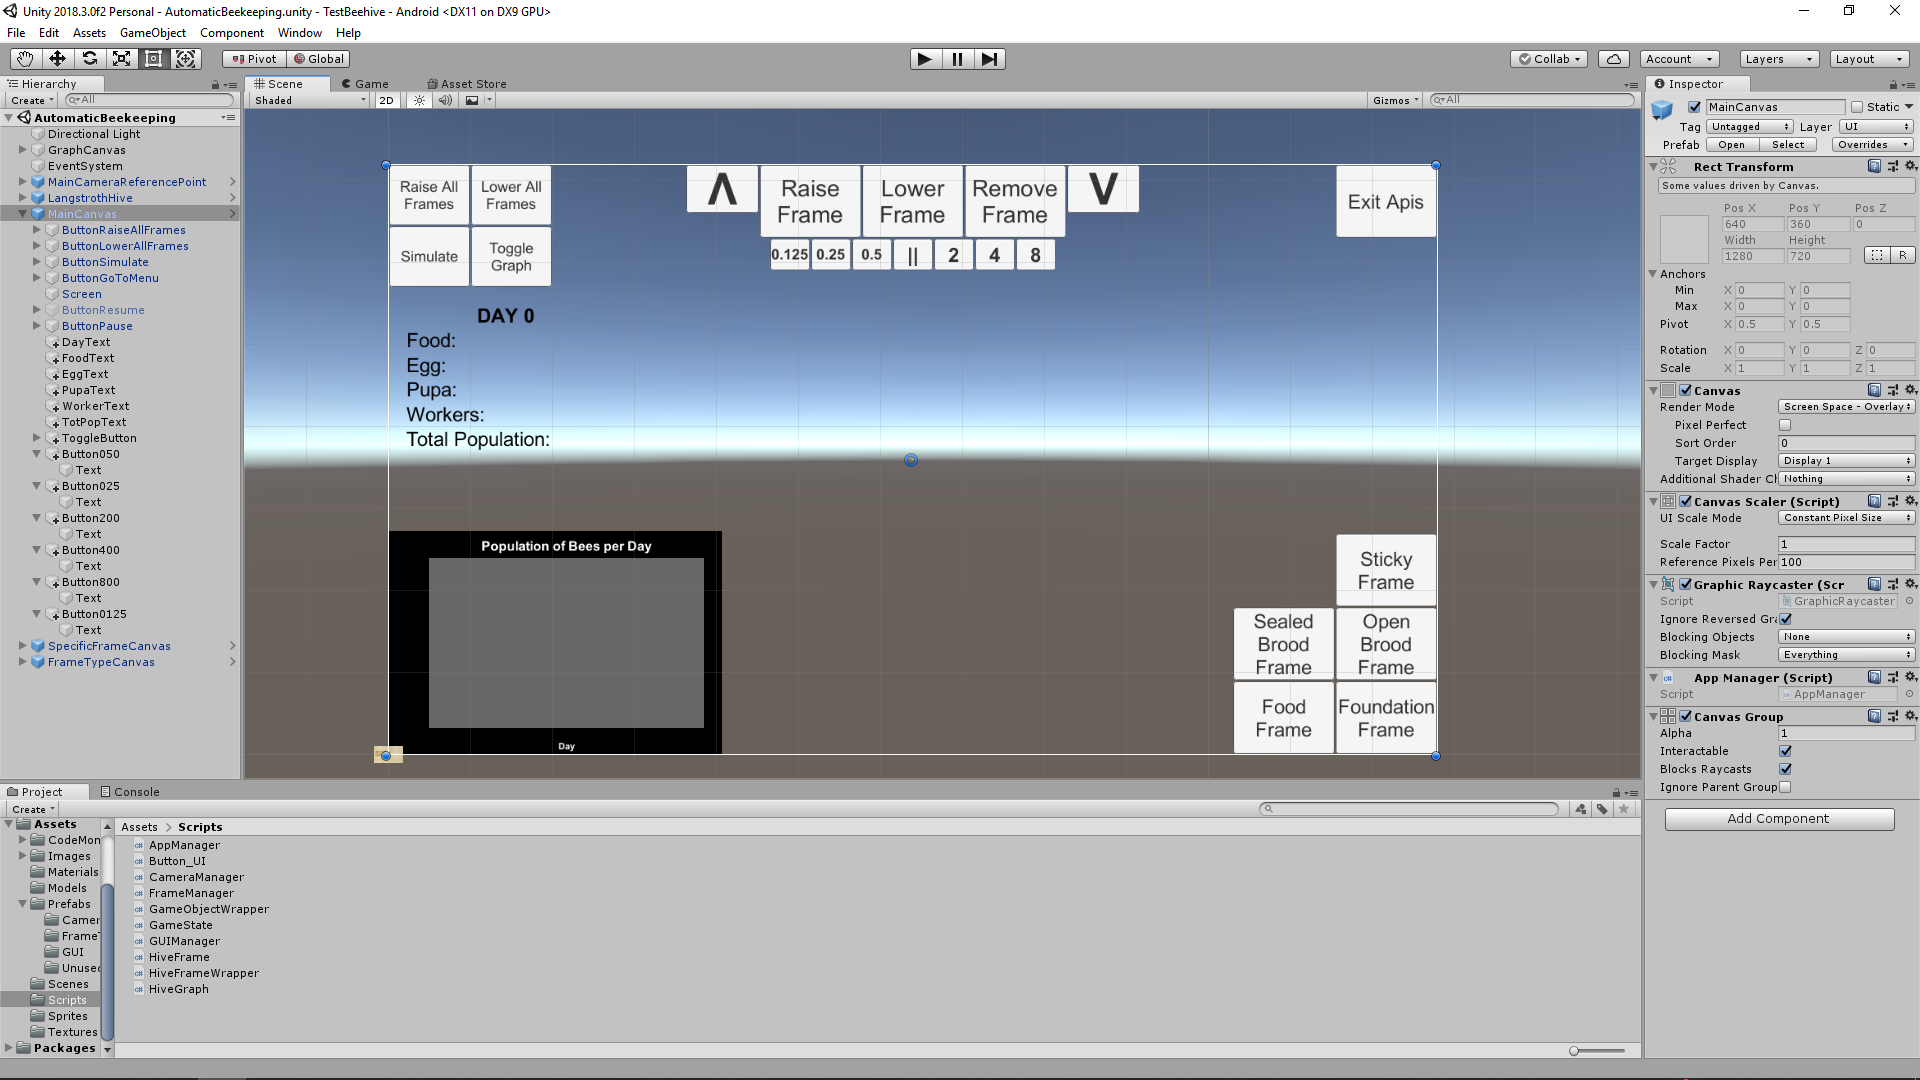
\includegraphics[scale=0.15]{./images/ui-auto-v2.png}
\centering
\caption{The development of Automatic Beekeeping UI}
\centering
\end{figure}

\begin{figure}[H]
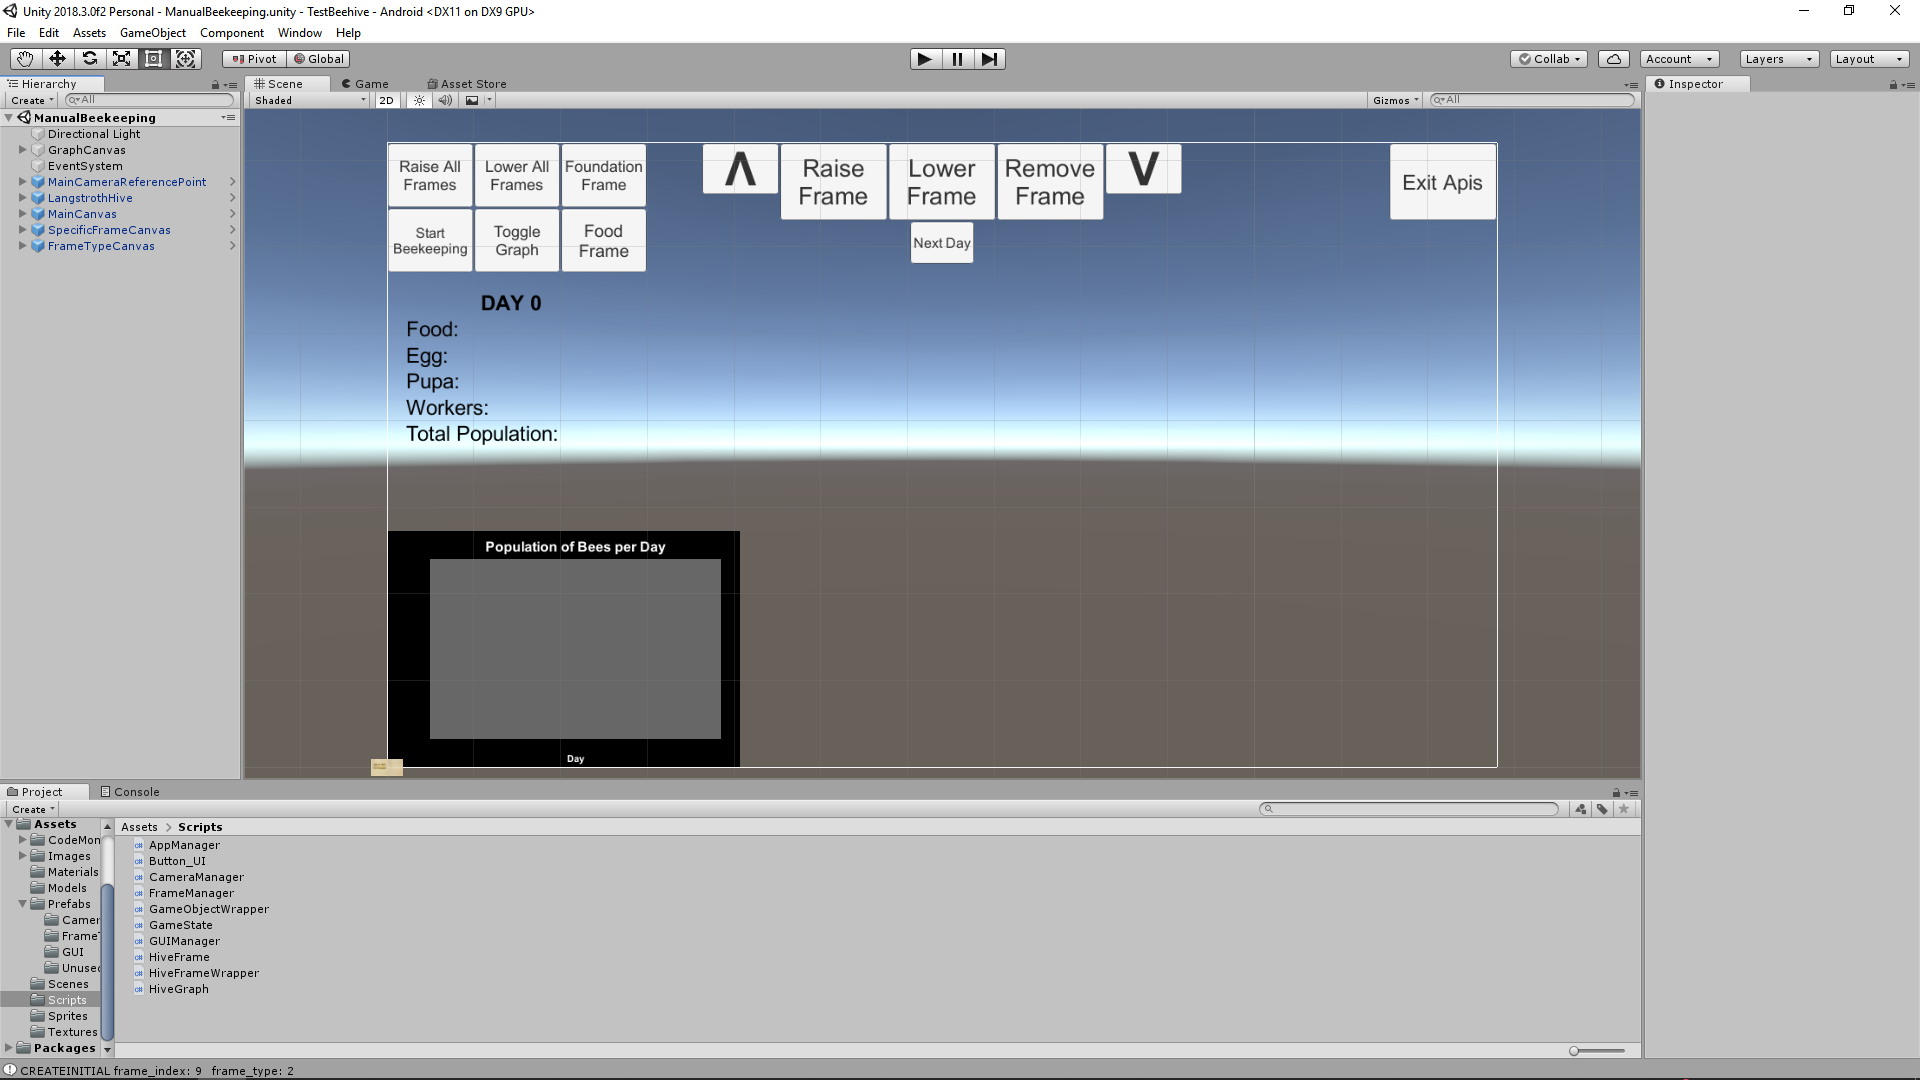
\includegraphics[scale=0.15]{./images/ui-manual.png}
\centering
\caption{The development of Manual Beekeeping  UI}
\centering
\end{figure}

\subsection{Implementation}
\indent The boxed hive model was created from a Blender-default 3D cube model. The model's top face was then removed. It was then cut into 4 sections to make the model creation more manageable. The model was molded and then applied with Mirroring operation. Afterwards, a texture map was created for the model. Revisions for the texture were done in MS PowerPoint 2013. Fig. 6 depicts the process of creating the boxed hive.
\begin{figure}[H]
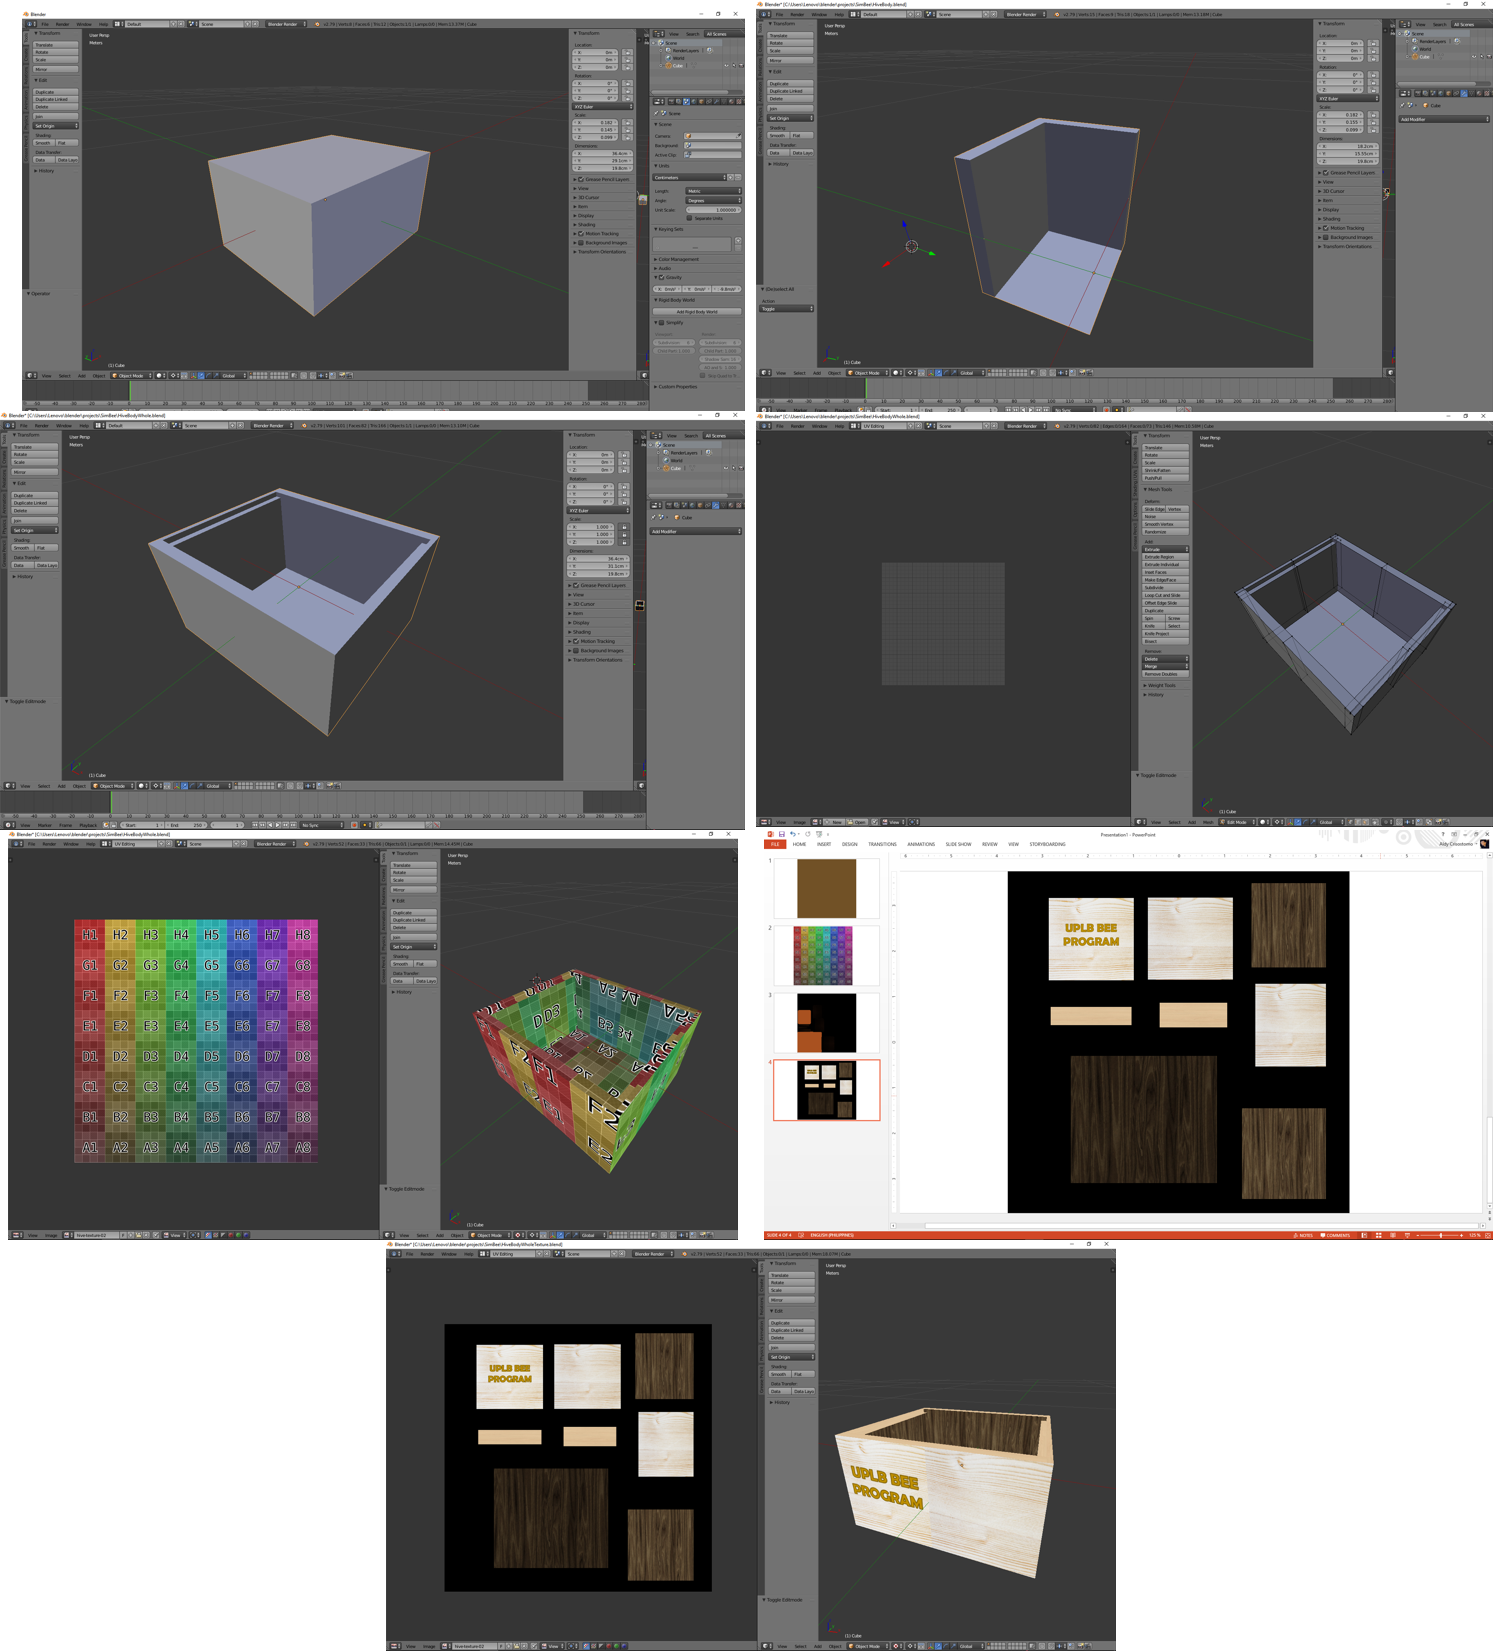
\includegraphics[scale=0.275]{./images/boxed-hive-model.png}
\centering
\caption{Creation process of Langstroth boxed hive model}
\centering
\end{figure}
\indent The same steps were also done for the wired frame. Fig. 7 shows the creation process for the wired Frame.
\begin{figure}[H]
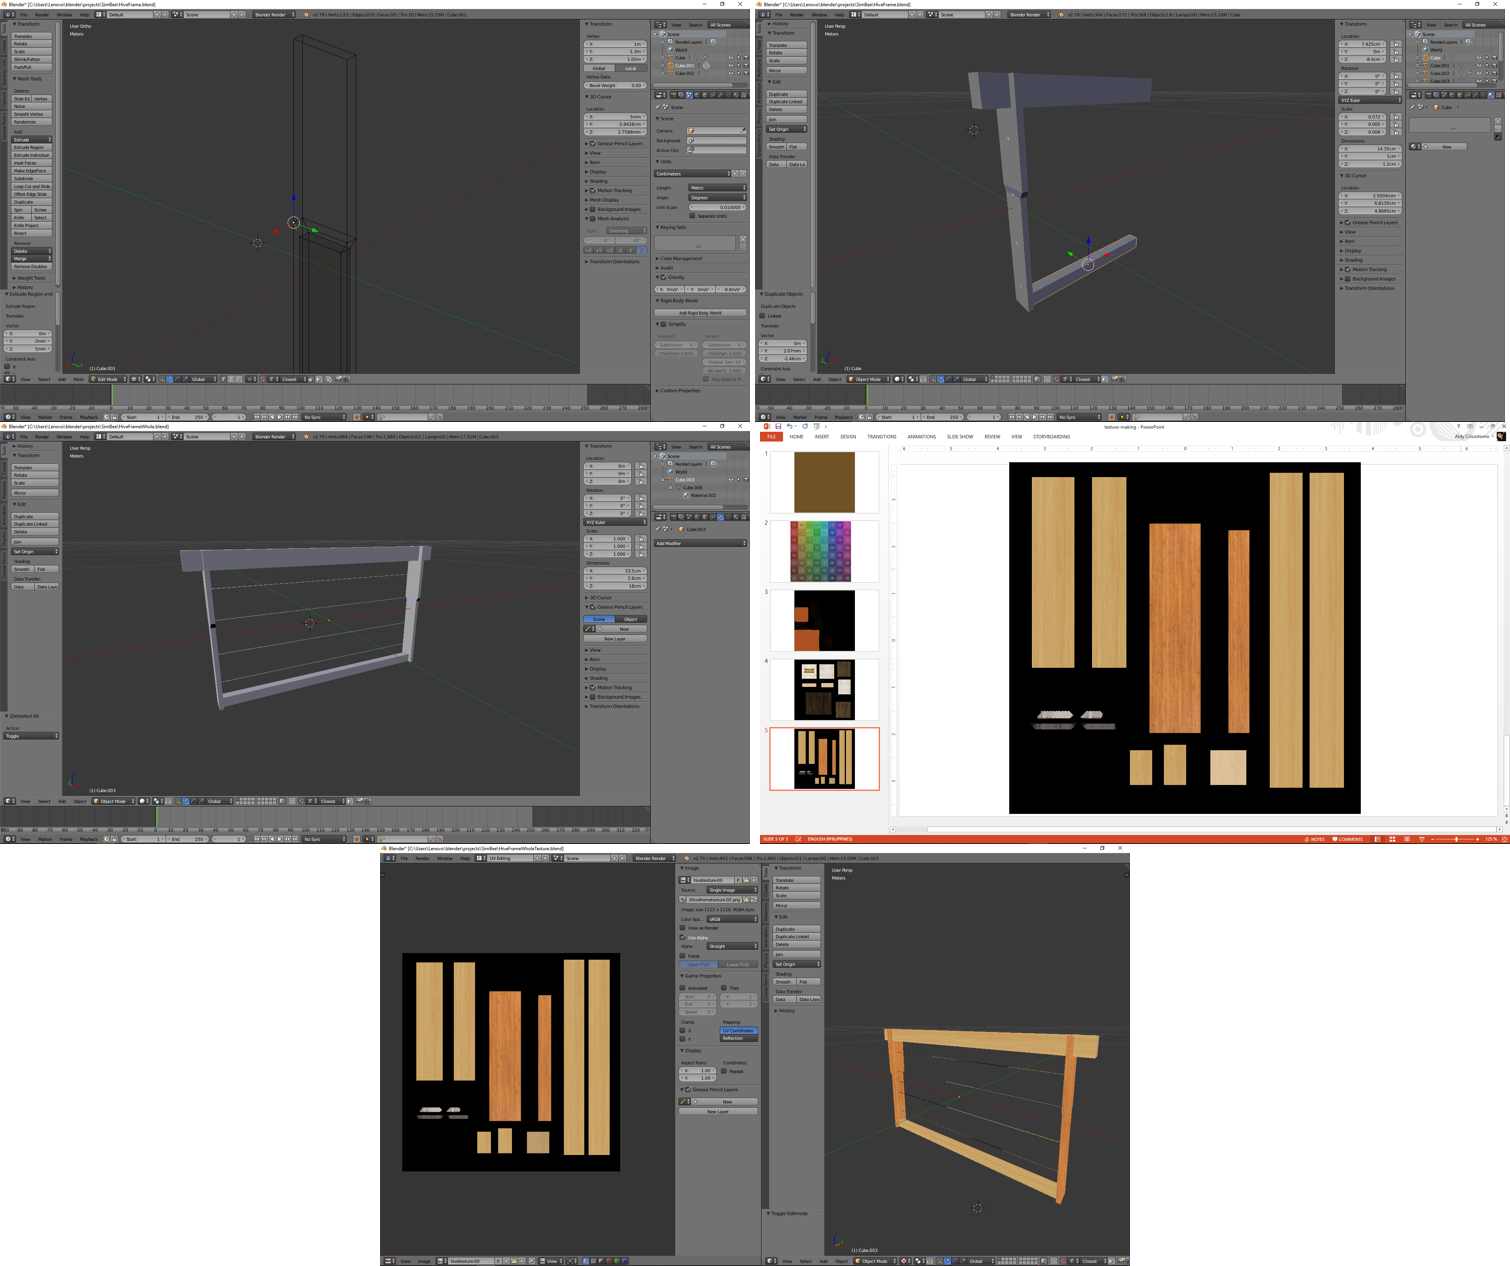
\includegraphics[scale=0.265]{./images/wired-frame-model.png}
\centering
\caption{Creation process of wired Frame model}
\centering
\end{figure}
\indent MS PowerPoint 2013 was used in creating the separate textures for the frame types, as seen in Fig. 8.
\begin{figure}[H]
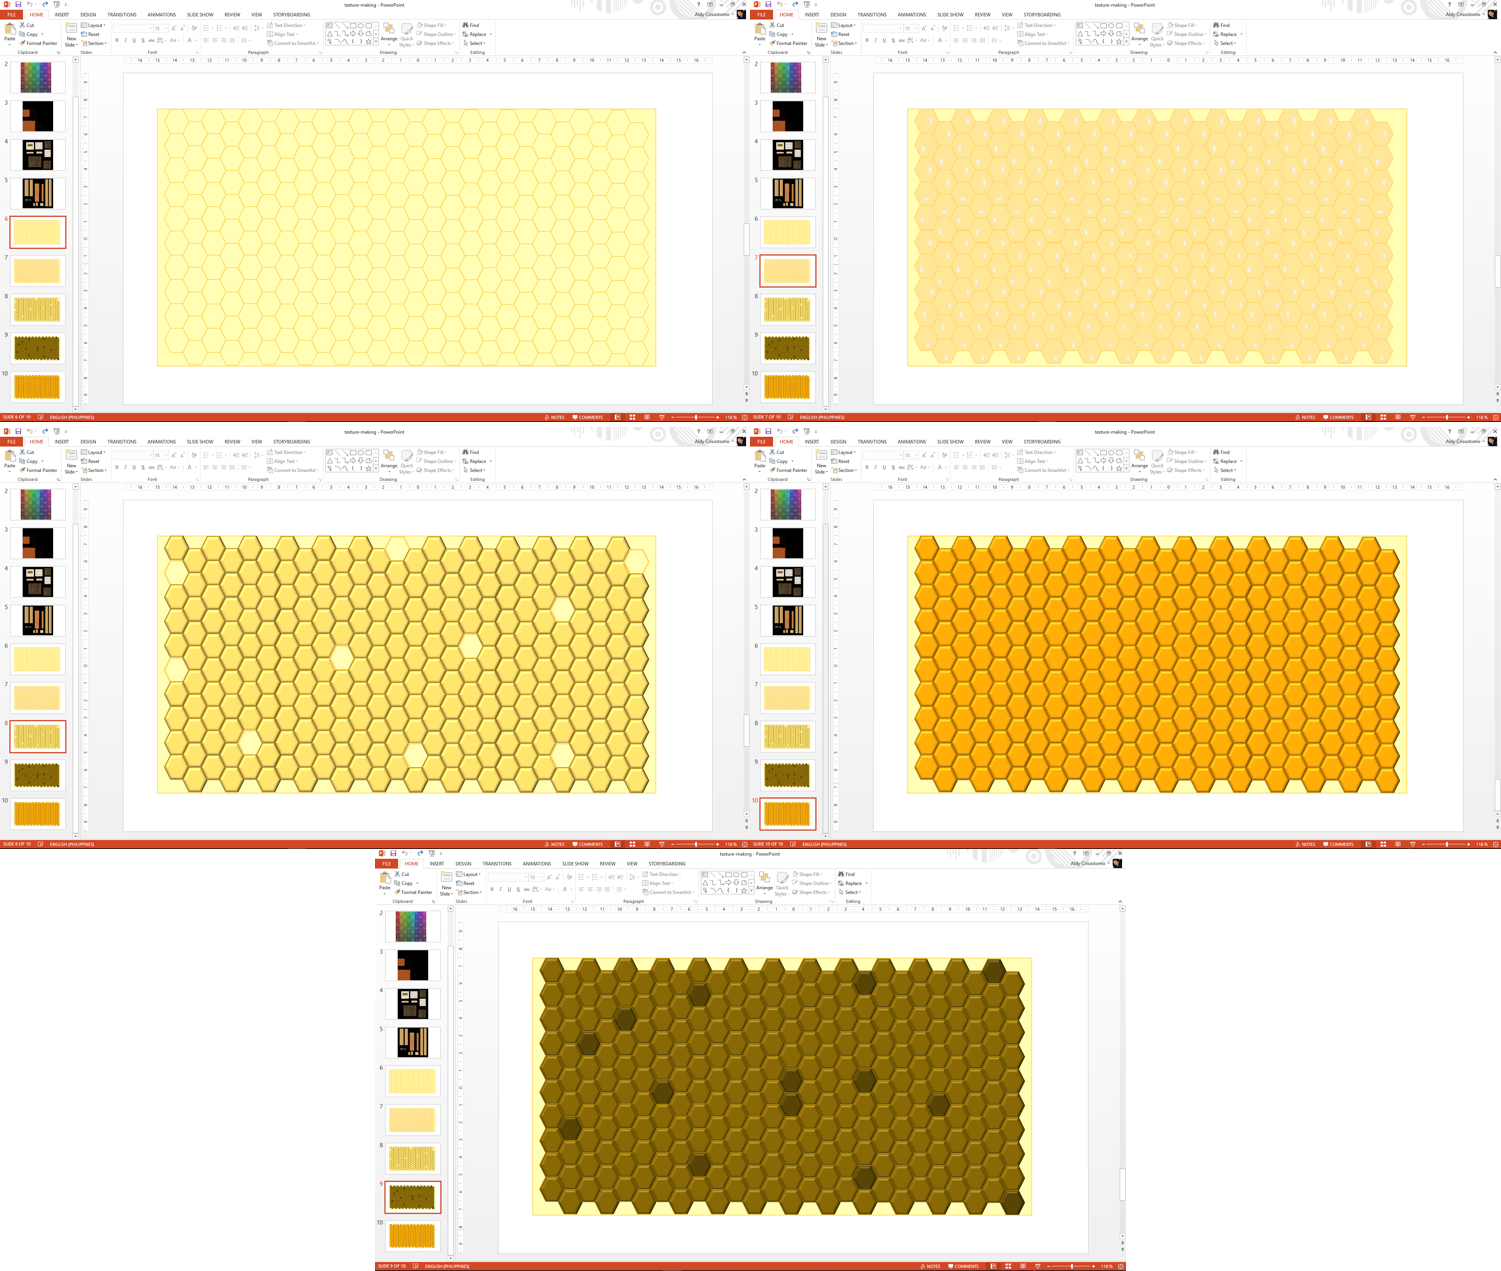
\includegraphics[scale=0.25]{./images/frame-type-textures.png}
\centering
\caption{From left-to-right: the Foundation frame, Open Brood Frame, Sealed Brood Frame, Sticky Frame, and Food frame}
\centering
\end{figure}

\indent The Unity game engine was used in developing the logic of the application along with the integration of the 3D models and textures. The drag-and-drop feature of the engine was utilized to design the UI elements of the simulation application. Fig. 9 shows the development process of the mobile application.
\begin{figure}[H]
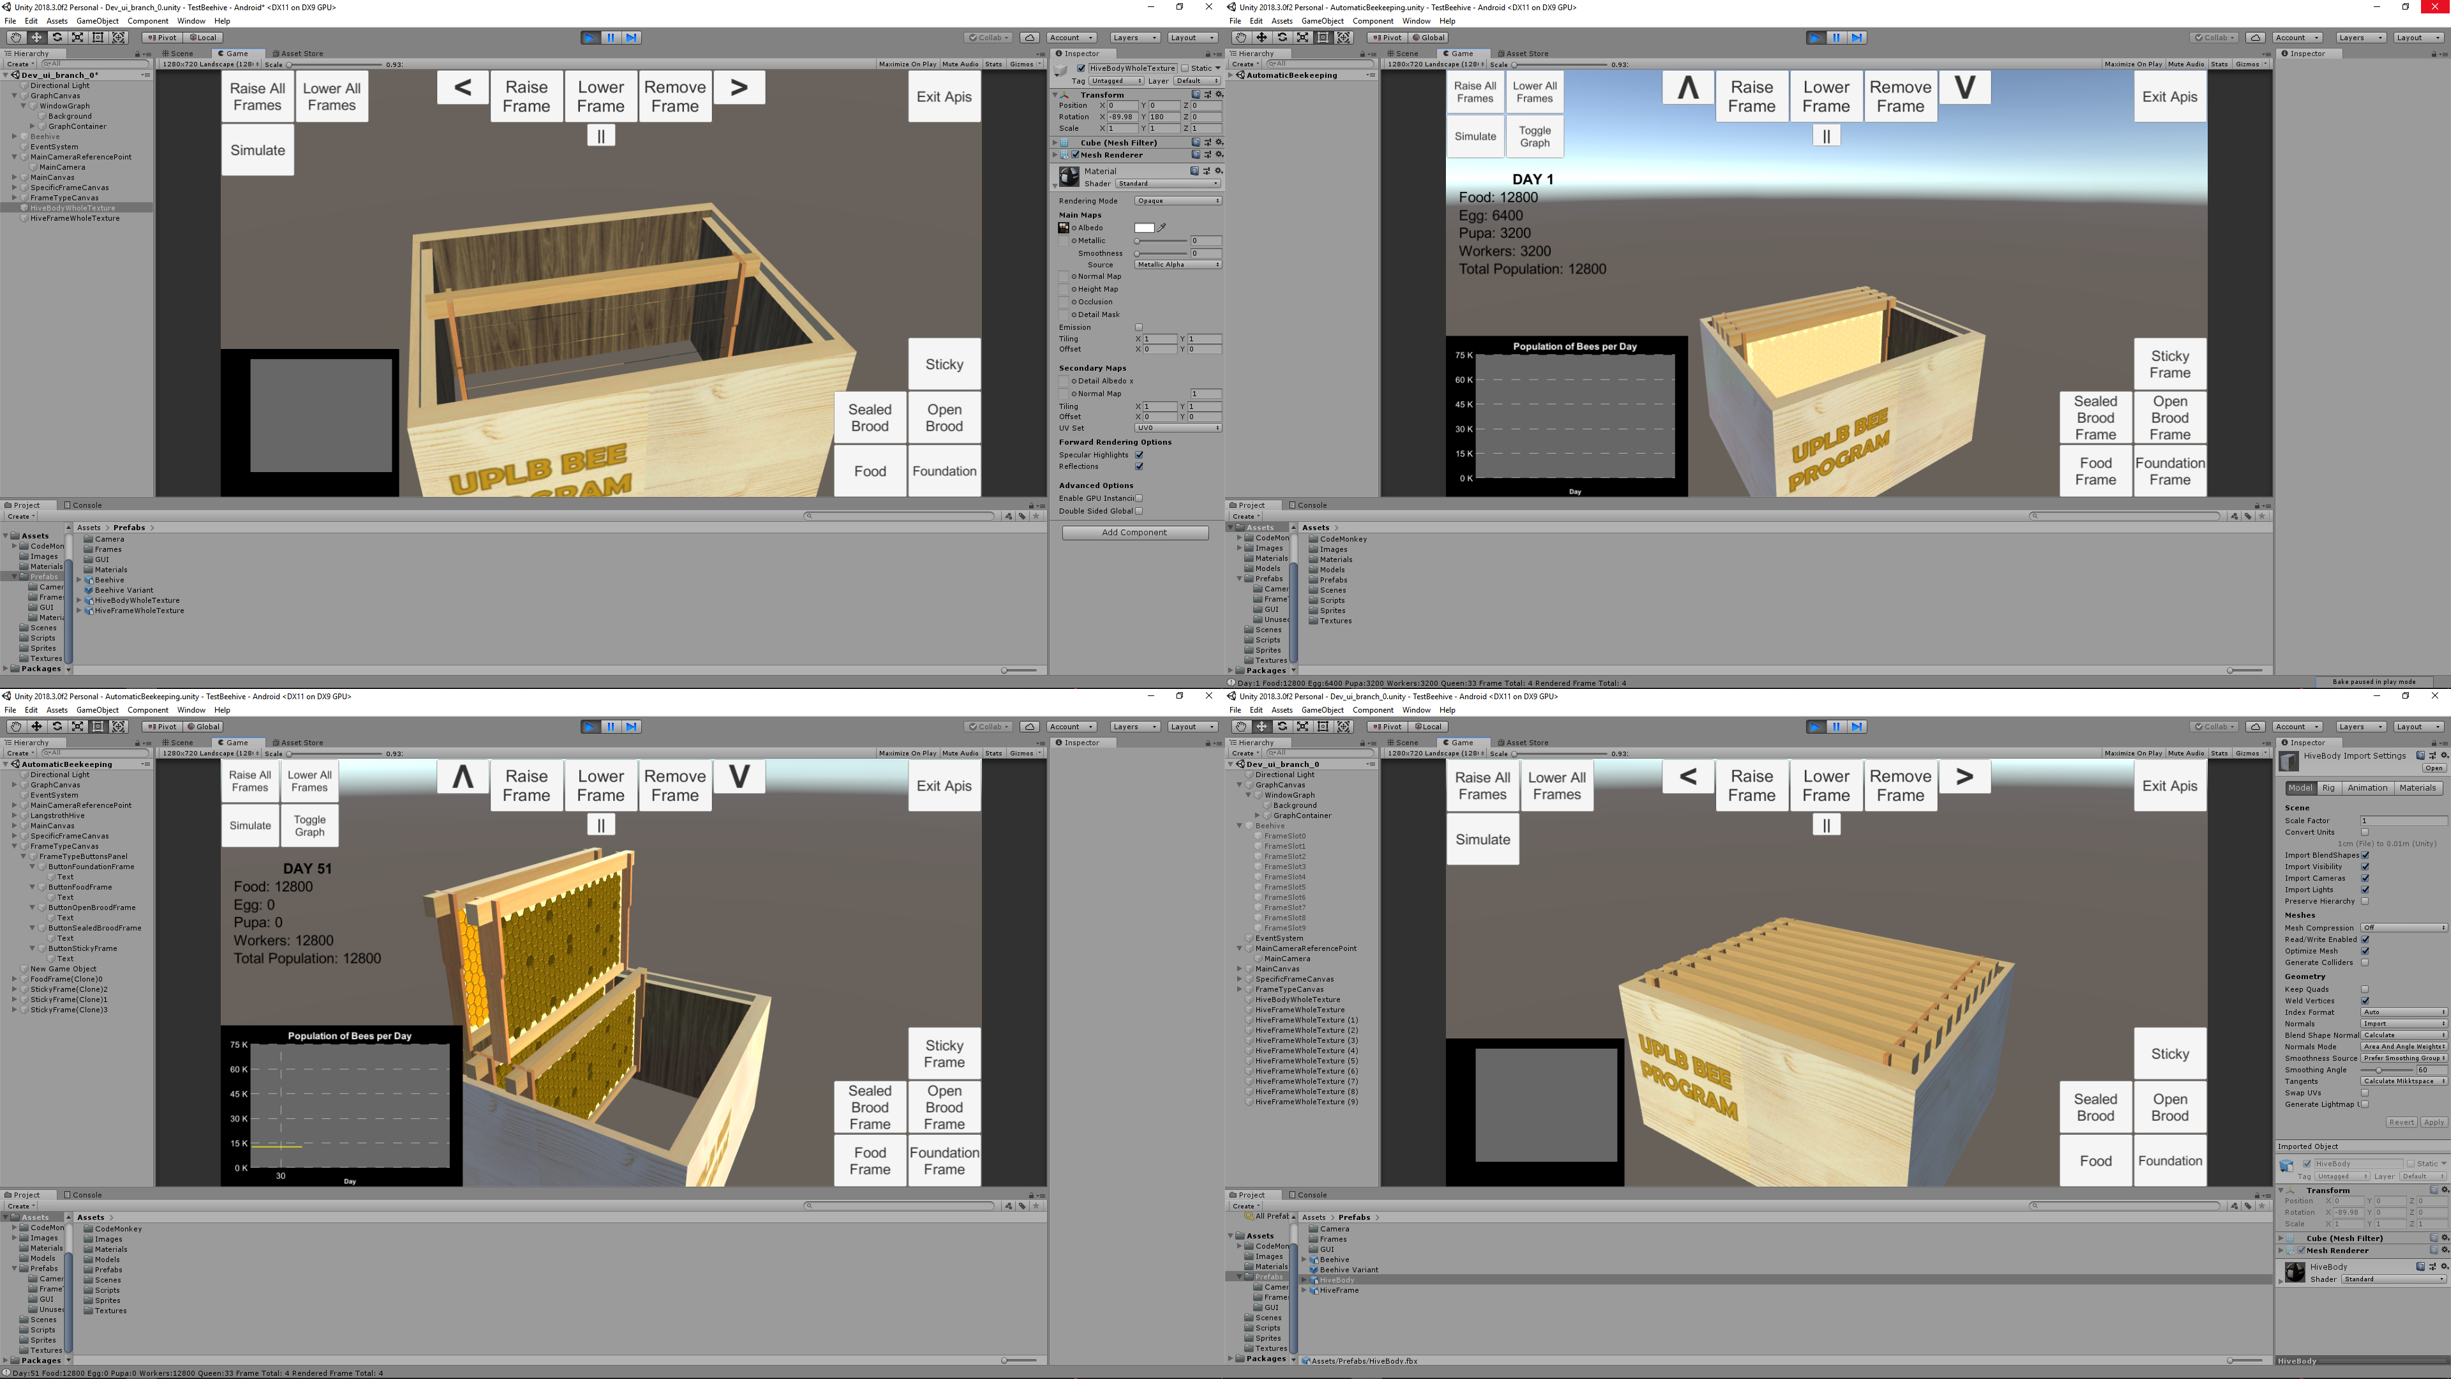
\includegraphics[scale=0.2]{./images/unity-dev-process.png}
\centering
\caption{The development process of the mobile application}
\centering
\end{figure}

% RESULTS AND DISCUSSION
\section{Results and Discussion}
\indent The researcher was able to abstract and create 3D models of the equipment used in seasonal beehive management, as shown in Fig. 10 and Fig. 11.
% Boxed Hive Model
\begin{figure}[H]
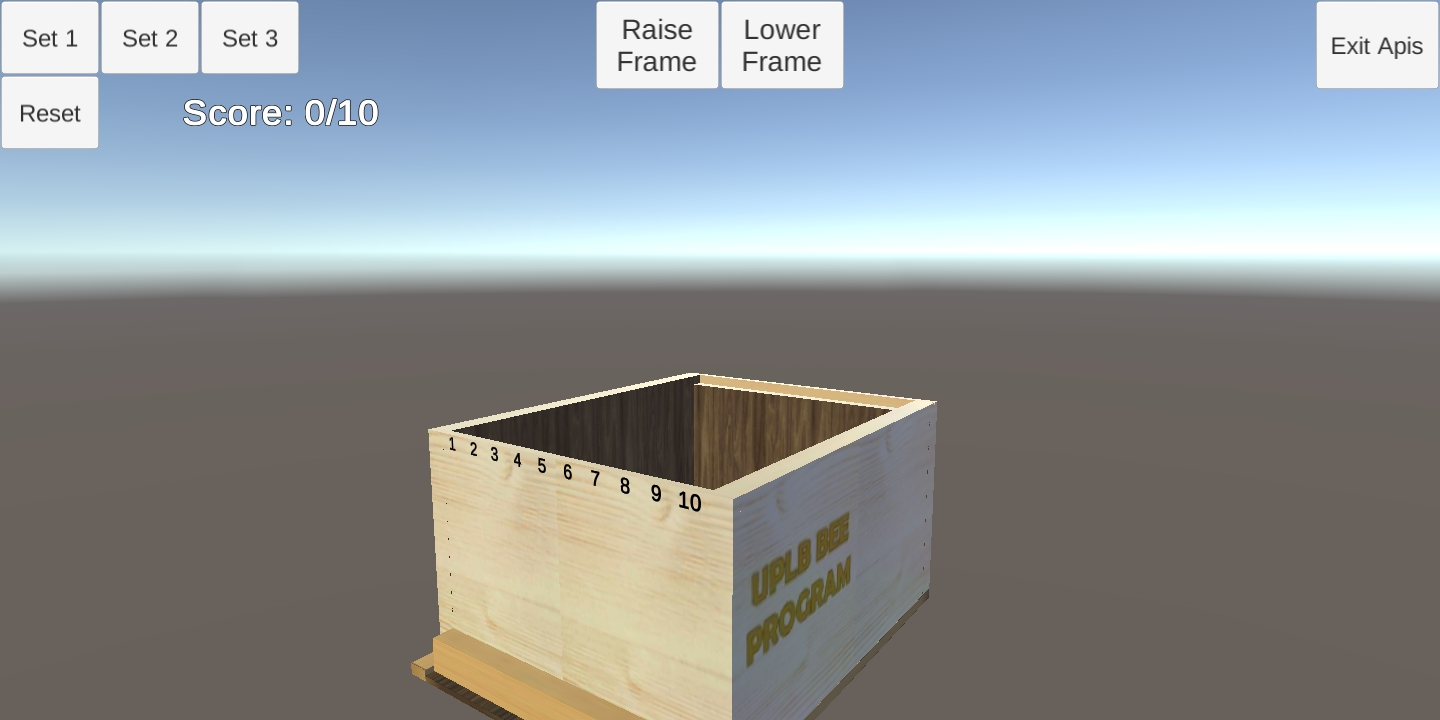
\includegraphics[scale=0.17]{./images/beehive-box-new.jpg}
\centering
\caption{3D model of the Langstroth boxed hive, housing different frame types}
\end{figure}
% Frame Type Models
\begin{figure}[H]
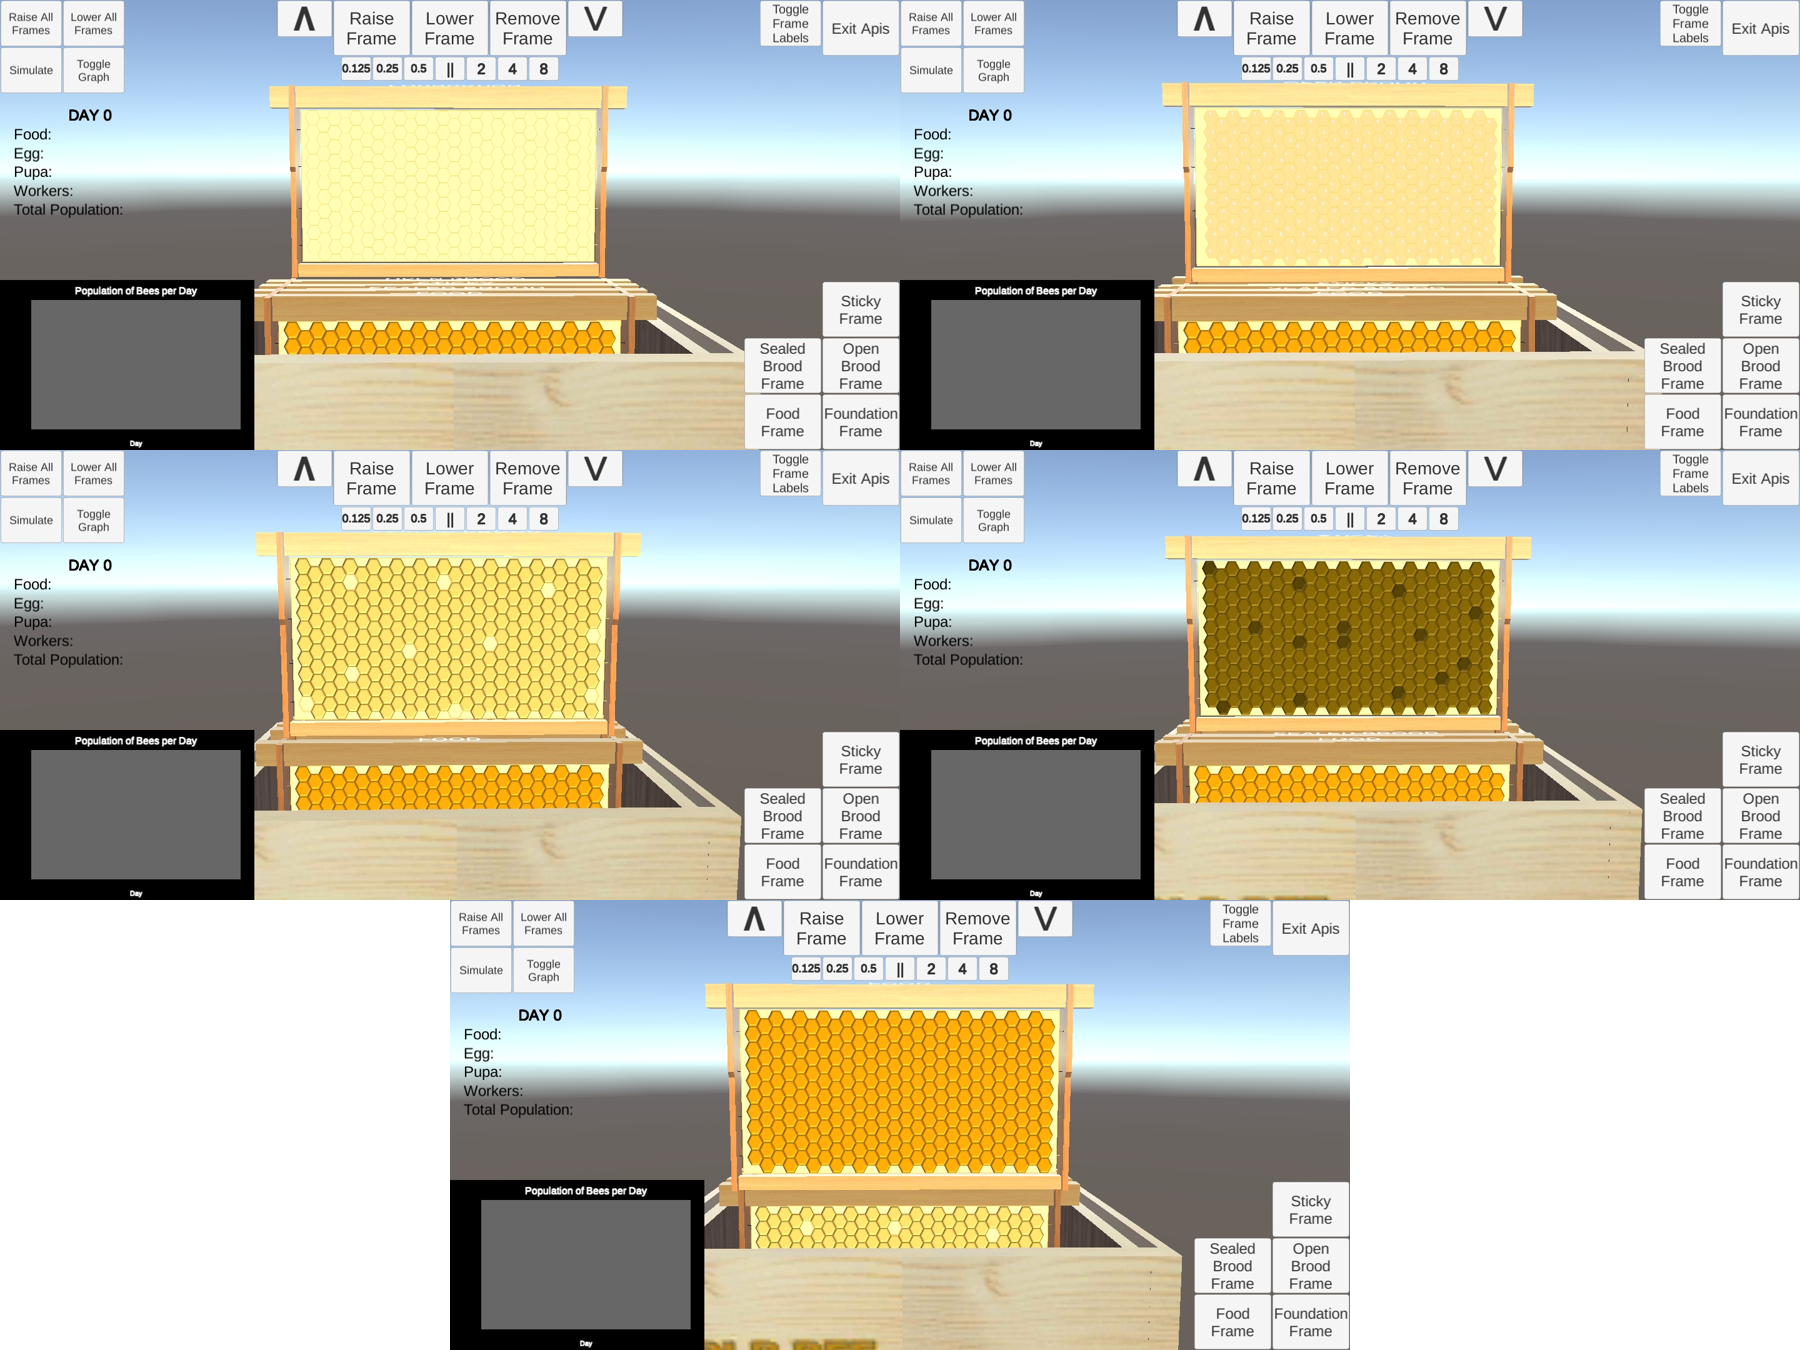
\includegraphics[scale=0.29]{./images/frame-types-new.png}
\centering
\caption{From left-to-right: Foundation Frame, Open Brood Frame, Sealed Brood Frame, Sticky Frame, and Food Frame}
\end{figure}
\indent The researcher was also able to develop a working main menu that can lead the user to either of the three modes of interaction: Quiz, Automatic Beekeeping, and Manual Beekeeping. Fig. 12 shows the Menu. Fig. 13, Fig. 14, and Fig. 15 show the use of the Quiz mode. Fig. 16 and Fig. 17 show the Automatic and Manual Beekeeping modes. 
\begin{figure}[H]
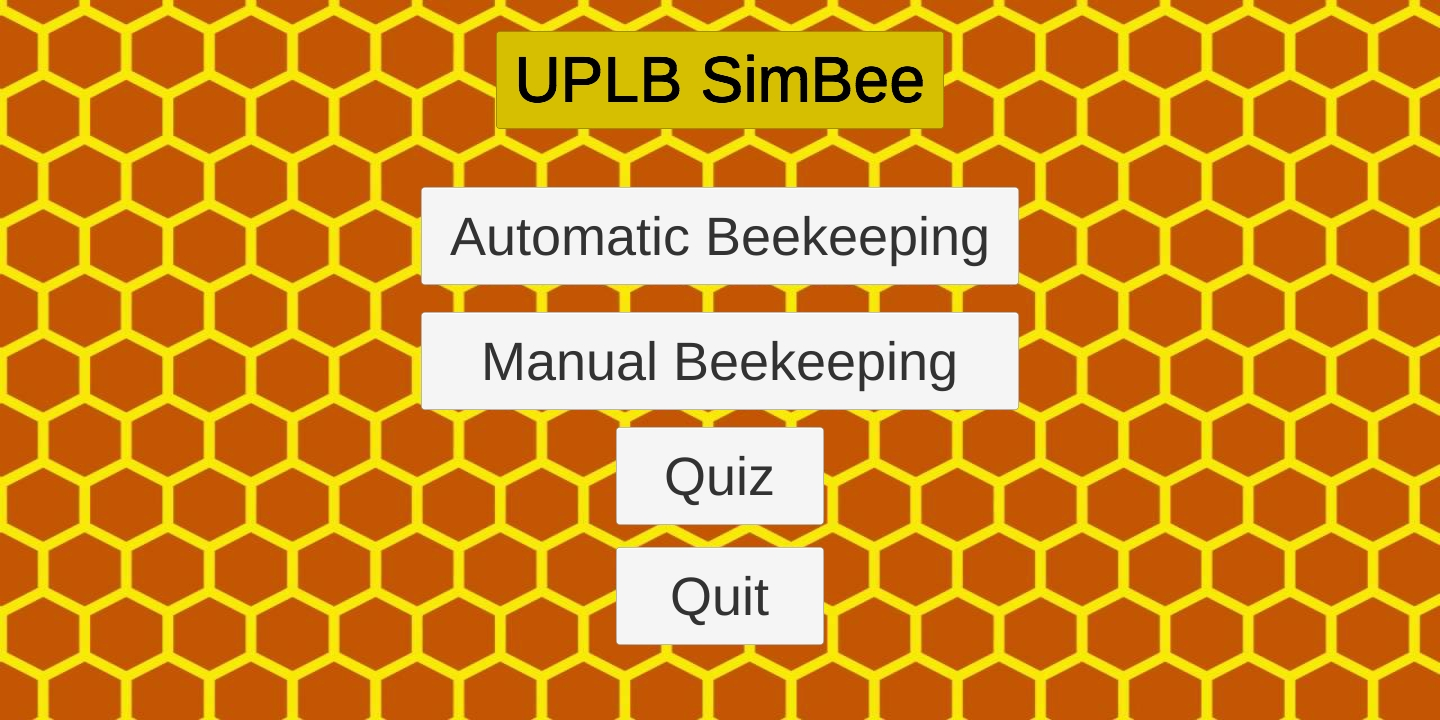
\includegraphics[scale=0.17]{./images/output-main-menu.jpg}
\centering
\caption{The main menu of the mobile application}
\end{figure}

\begin{figure}[H]
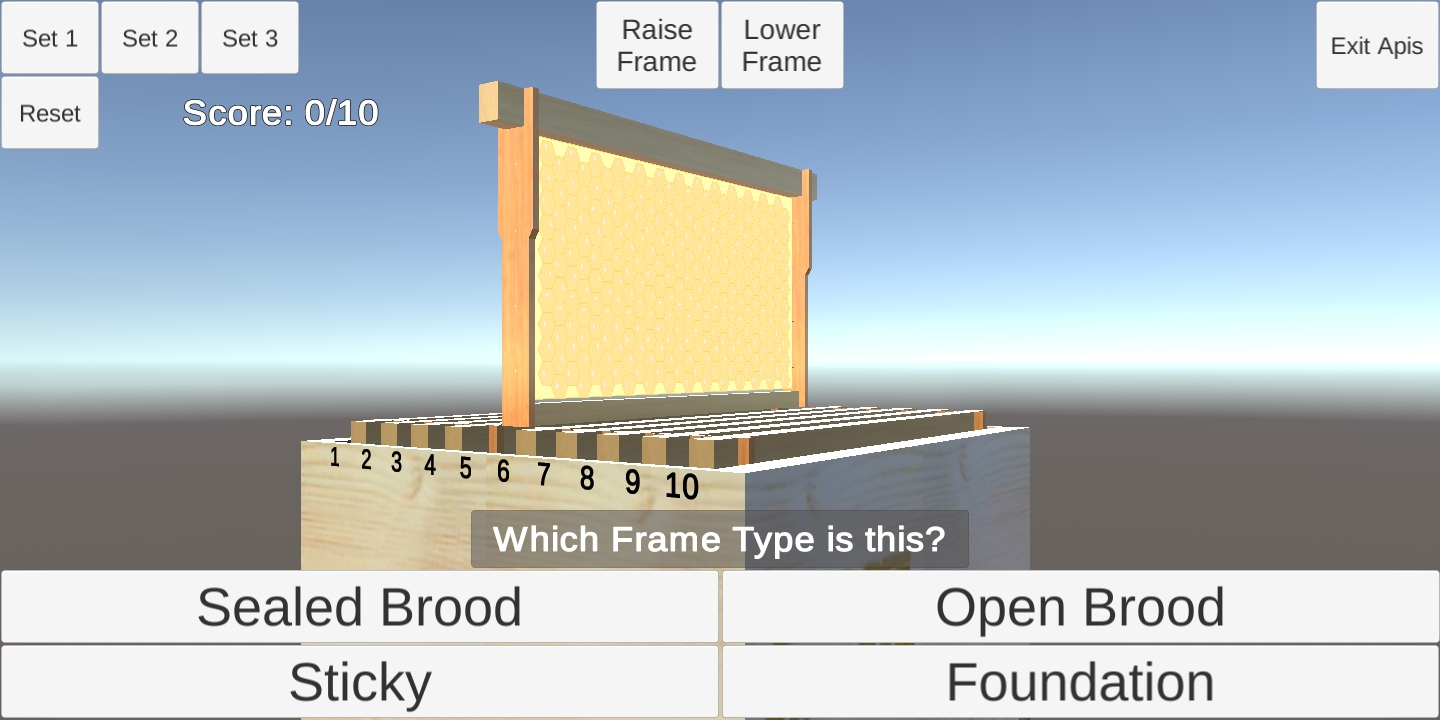
\includegraphics[scale=0.17]{./images/quiz-game-1.jpg}
\centering
\caption{A user attempting to answer a Quiz item}
\end{figure}

\begin{figure}[H]
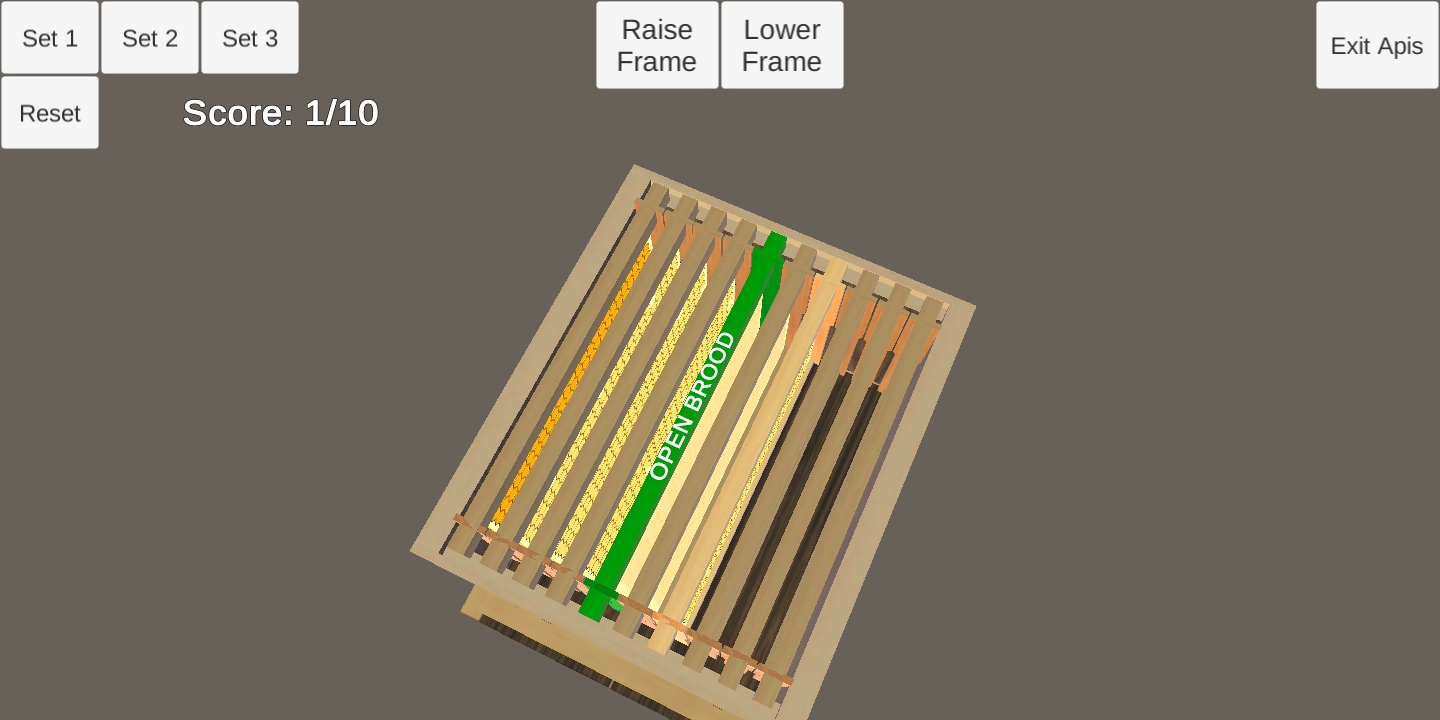
\includegraphics[scale=0.17]{./images/quiz-game-2.jpg}
\centering
\caption{A green frame after giving a correct answer}
\end{figure}

\begin{figure}[H]
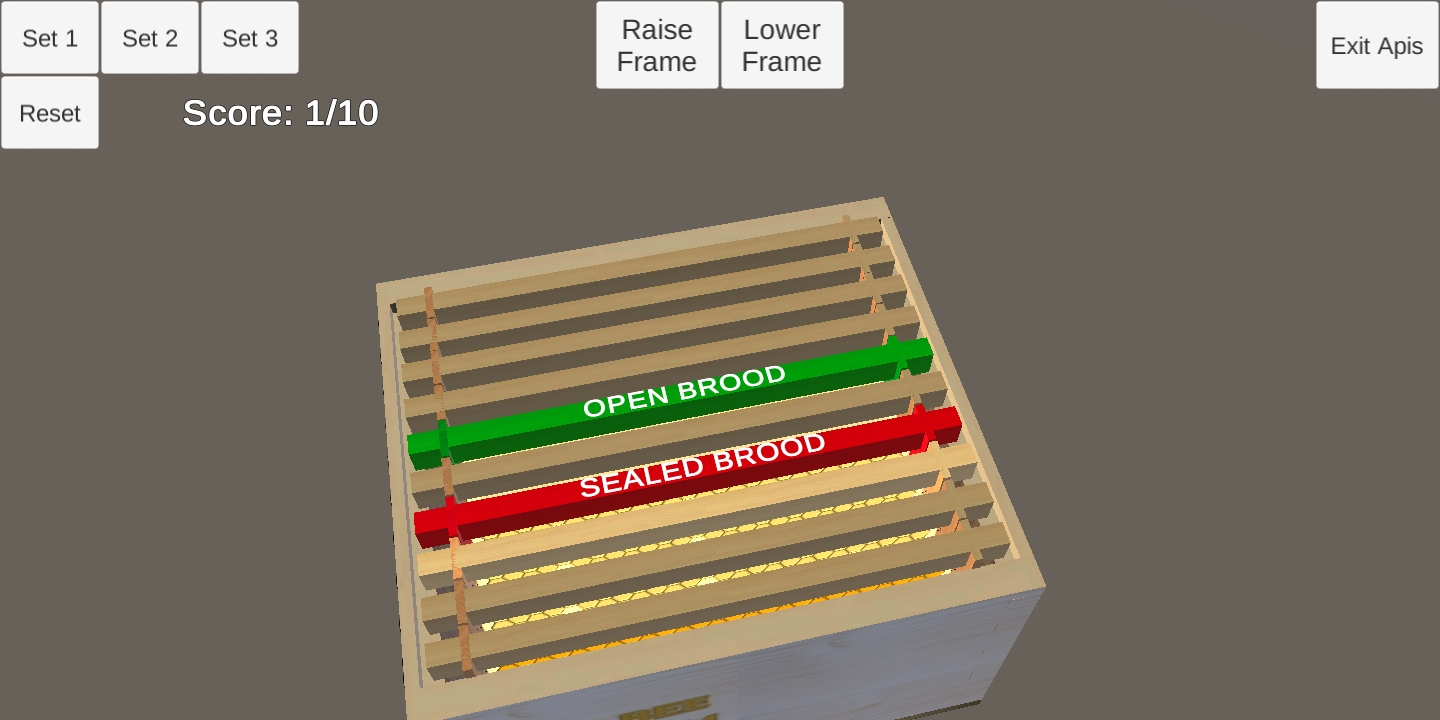
\includegraphics[scale=0.17]{./images/quiz-game-3.jpg}
\centering
\caption{A red frame after giving a wrong answer}
\end{figure}

\begin{figure}[H]
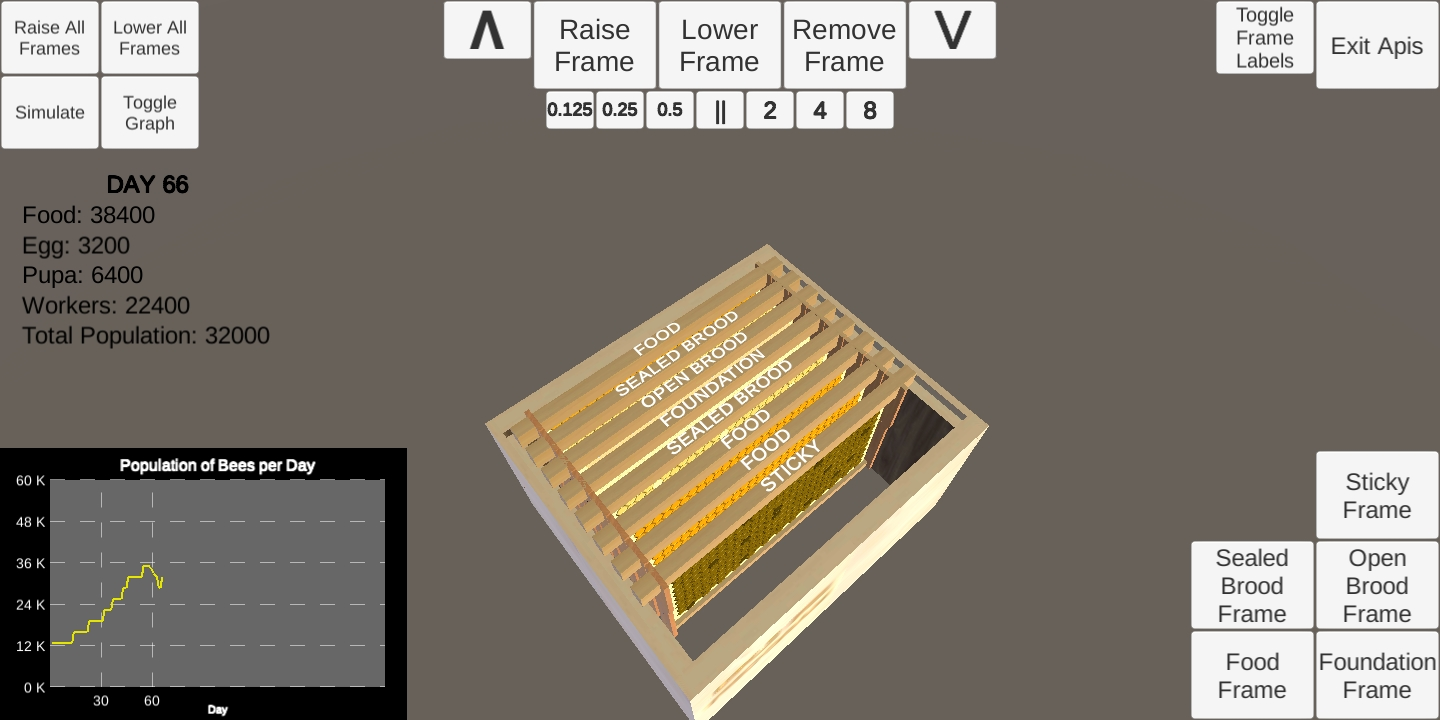
\includegraphics[scale=0.17]{./images/automatic-beekeeping-new.jpg}
\centering
\caption{The Automatic Beekeeping mode}
\end{figure}

\begin{figure}[H]
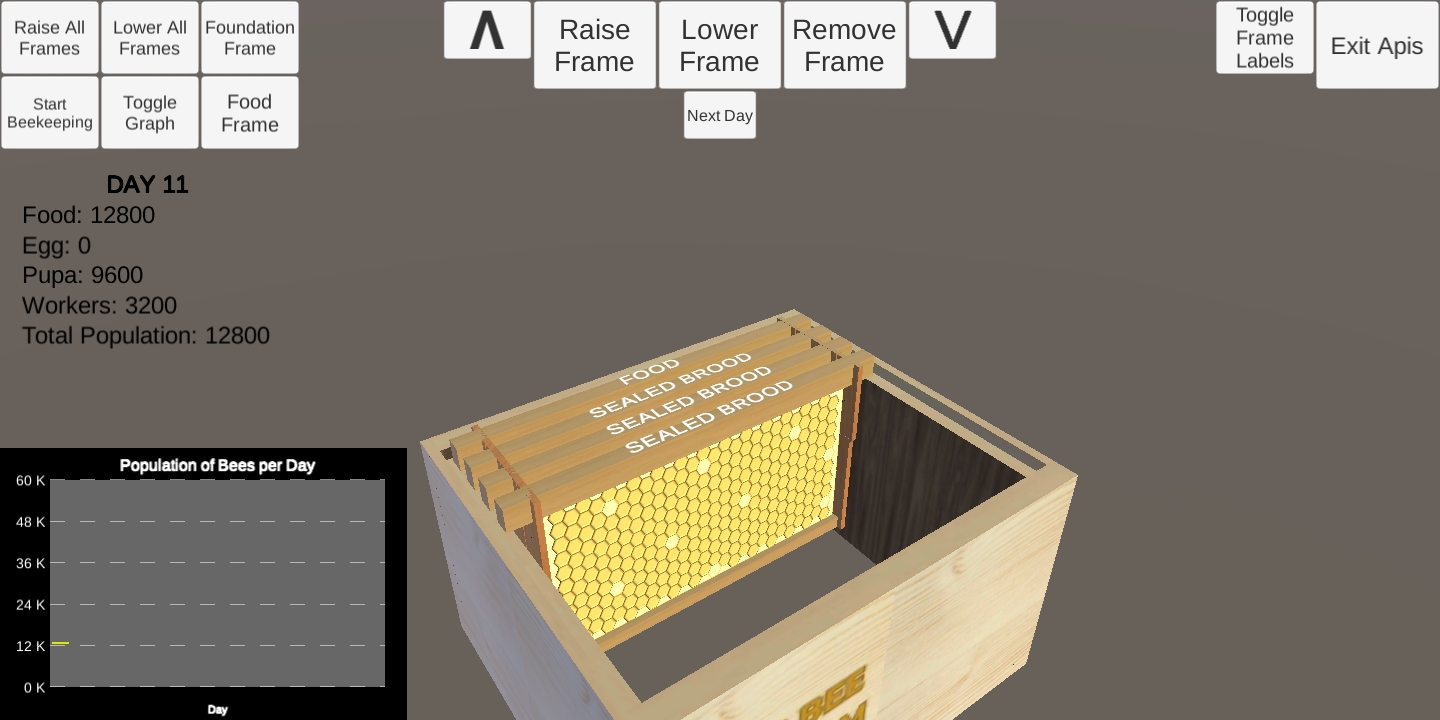
\includegraphics[scale=0.17]{./images/manual-beekeeping-new.jpg}
\centering
\caption{The Manual Beekeeping mode}
\end{figure}

\indent The simulation model follows the proper seasonal beekeeping setup. The hive starts with a Food Frame, an Open Brood Frame, a Sealed Brood Frame and an Open Brood Frame placed in that order. The first season is July-December and prioritizes brood expansion. If there are no more frames to lay eggs in or gather food in, a foundation frame is added until there are 10 frames. New sticky frames for expanding brood is relocated to the relative center of the hive for the queen to lay eggs into.
\newline
\indent Fig. 18 shows an automatic simulation of proper seasonal beehive management. The yellow line graph shows the progression of the bee population as in-app days go on.
\begin{figure}[H]
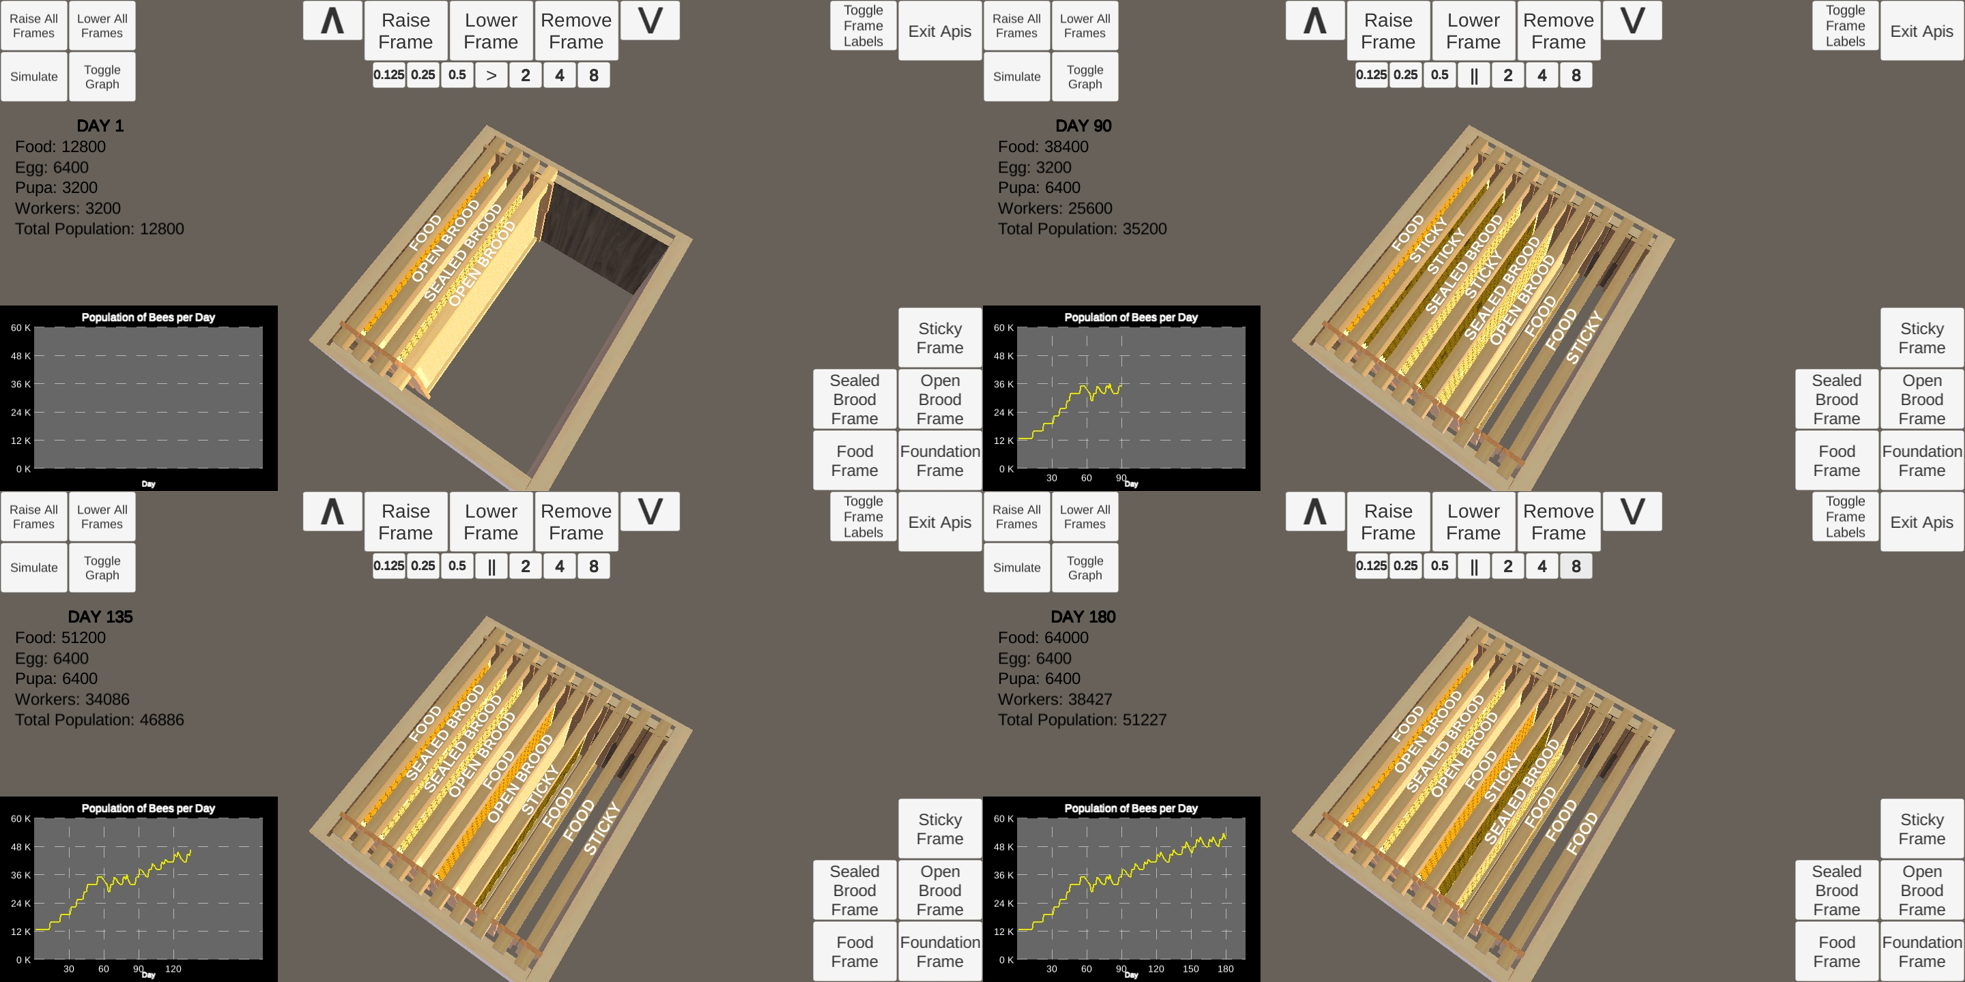
\includegraphics[scale=0.2625]{./images/automatic-proper-mgt.png}
\centering
\caption{Image sequence depicting proper beehive management}
\end{figure}
An improper practice of beehive management was demonstrated in the application. Sticky frames were relocated in an unsuitable frame slot within the first few in-app days. The outcome was reflected in the red line graph, as shown in Fig. 19.
\begin{figure}[H]
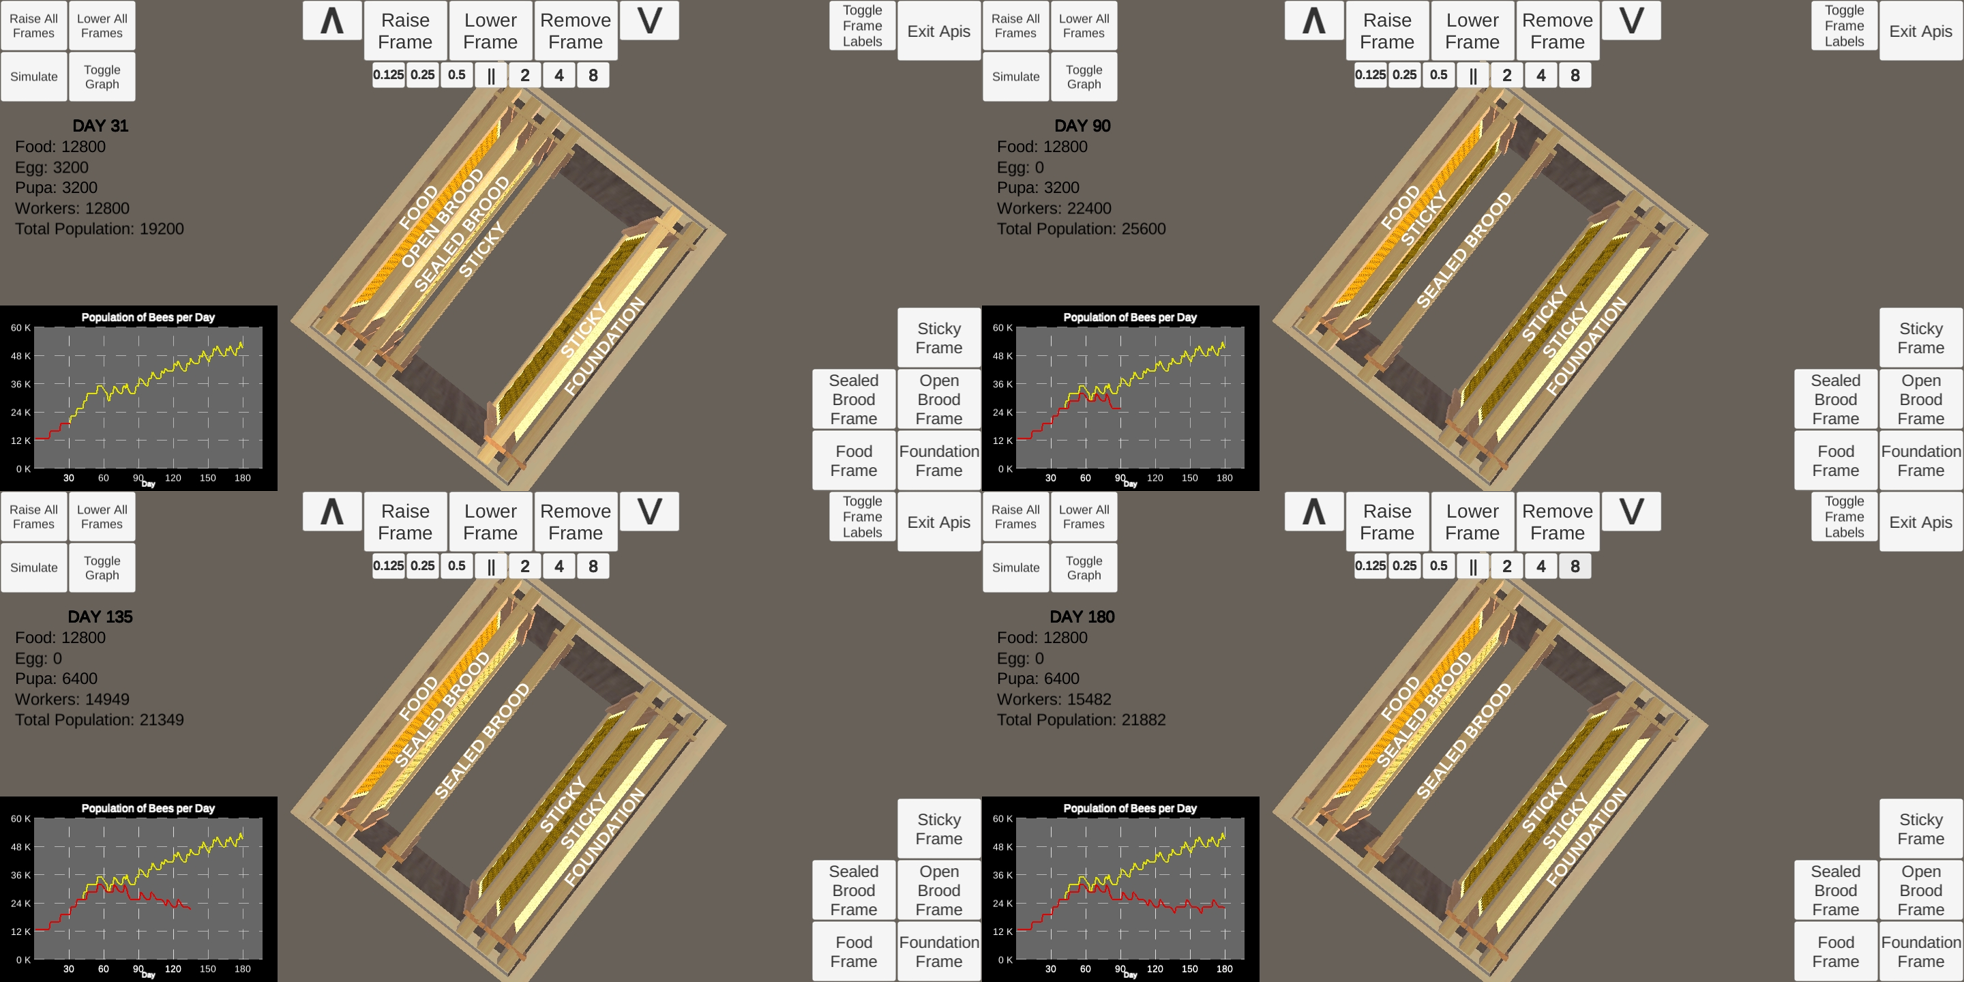
\includegraphics[scale=0.2625]{./images/automatic-improper-mgt.png}
\centering
\caption{Image sequence depicting improper beehive management}
\end{figure}

% CONCLUSION
\section{Conclusion}
 The researcher was able to create 3D models of the equipment used for beekeeping. The researcher was successful in developing a working mobile simulation application about proper seasonal beehive management. Multiple scenes were also developed to cater for different purposes of using the mobile simulation app, such as the Quiz, Automatic Beekeeping, and Manual Beekeeping. 

% RECOMMENDATIONS
\section{Recommendations}
The mobile simulation application was able to simulate beehive management and show the outcomes of users interacting with the hive. The researcher recommends the following for the improvement of the mobile application:
\begin{itemize}
    \item Improve the accuracy and precision of the simulation logic.
    \item Create more intricate textures for individual hive cells, such that it more accurately reflects the data of the cells in each frame.
    \item Improve the look-and-feel of the user interface such that interaction with the hive is made easier for general users.
    \item Include environmental conditions and bee diseases that can affect the collective growth and strength of the Langstroth beehive.
\end{itemize}

% BIBLIOGRAPHY
\bibliographystyle{./IEEE/IEEEtran}
%\bibliography{./cs190-ieee}
% \nocite{*}
\begin{thebibliography}{13}

\bibitem{agera}
Agera, S.I.N. (2011). Role of beekeeping in the conservation of forests. \textit{Global Journal of Agricultural Sciences, 10}(1), 27-32. Retrieved from https://www.ajol.info/index.php/gjass/article/viewFile/79068/69377

\bibitem{bradbear}
Bradbear, N. (2009). Bees and their role in forest livelihoods. \textit{A Guide to the Services Provided by Bees and the Sustainable Harvesting, Processing and Marketing of Their Products}. Retrieved from http://www.fao.org/3/a-i0842e.pdf

\bibitem{barbosa}
Barbosa, H. (2015). 3D simulation environment: education and training. In \textit{Proceedings of the 10th Doctoral Symposium in Informatics Engineering}, 132-133. Retrieved from https://www.researchgate.net/publication/319220185\_3D\_Simulation
\newline\_Environment\_Education\_and\_Training
    
\bibitem{cervanciaetal}
Cervancia, C.R., Fajardo, A.C., Jr., Manila-Fajardo, A.C., \& Lucero, R.M. (2012). Management of Philippine Bees: Stingless Bees and Honey Bees with Bibliography of Philippine Bees. Los Banos, Laguna: University of the Philippines Los Banos Bee Program

\bibitem{clarino}
Clari\~{n}o, M. D. (2013). \textit{3D seasonal beehive management simulation} (undergraduate special problem). University of the Philippines Los Baños, Laguna, Philippines

\bibitem{heier}
Heier, C. (2015). Free to play: mobile gaming and the precipitous rise of freemium. In \textit{The Review: A Journal of Undergraduate Student}, \textit{16}(4), 1-2. Retrieved from http://fisherpub.sjfc.edu/ur/vol16/iss1/4

\bibitem{beekeepingtraining}
Intensive Beekeeping Training Seminar. (2015). Retrieved from https://www.pinoybeekeepersforum.com/2015/11/04/intensive-beekeeping-training/

\bibitem{uplbbeeprogram}
Institute of Biological Sciences, UPLB. (2013). \textit{UPLB Bee Program} [PDF file] (para. 1). Retrieved from https://aboutphilippines.org/files/uplbbee.pdf

\bibitem{naziretal}
Nazir, N., Iqbal, M. A., Sarwar, A., & Altaf, M. N. (2011). Modern simulation and modeling techniques used For virtual object animations. In \textit{International Journal of Advanced Research in Computer Science}, \textit{2}(2), 66. Retrieved from http://www.ijarcs.info/index.php/Ijarcs/article/download/364/354

\bibitem{santosaetal}
Santosa, H., Ikaruga, S., & Kobayashi, T. (2016). 3D interactive simulation system (3DISS) using multimedia application authoring platform for landscape planning support system. In \textit{CITIES 2015 International Conference, Intelligent Planning Towards Smart Cities}, Surabaya, Indonesia, 248. Retrieved from https://www.sciencedirect.com/science/article/pii/S1877042816307534

\bibitem{serrano}
Serrano, K. J. V. (2011). \textit{Computer simulation tool for the proper bee hive management training module} (undergraduate special problem). University of the Philippines Los Baños, Laguna, Philippines.

\bibitem{sugimuraetal}
Sugimura,  R., Kawazu, S., Tamari,  H., Watanabe,  K., Nishimura, Y.,Oguma,  T., & Inoue,  H.  (2014). Mobile game for learning bacteriology. In \textit{10th International Conference Mobile Learning}, 285. Retrieved from https://files.eric.ed.gov/fulltext/ED557221.pdf.

\bibitem{uplbbeeprogramsite}
UPLB Bee Program. (2014). Retrieved from https://idsc.uplb.edu.ph/agriculture-cluster/bee-program
\end{thebibliography}

% BIOGRAPHY
\begin{biography}[{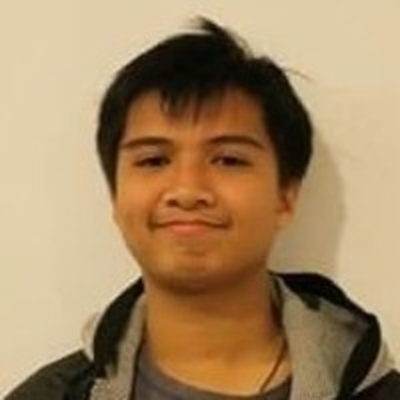
\includegraphics[scale=0.175]{./images/my-pic.png}}]{Albert Dominic Crisostomo}
is an undergraduate student under the BS Computer Science program of the University of the Philippines Los Ba\~{n}os. He loves playing video games and aspires to be a game developer.
\end{biography}


\end{document}
 
